\chapter{Transformation}\label{ch:transformation}
{
    \section{Introduction}
     {
      As previously discussed (see Chapter \eqref{ch:insight}), the role of insights is to focus the urban discussion on specific challenges, and establish clear KPIs to evaluate future interventions. The next step is to introduce and evaluate change to the city, in the from of urban \textit{Transformation}: an iterative exploration of design interventions and policies, set to transfer the city from its current state to another. In CityScope, evaluating transformation is possible through a wide range of Urban Human Computer Interaction (UHCI) methodologies, systems, and interfaces. Unlike traditional city-planning practices, CityScope is built for synchronous design exploration, in which evaluation of many design proposals is conducted simultaneously, while being fed by real-time data and analysis. To achieve this capability, CityScope has two main streams of development: (i) \textbf{CityScope UHCI:} The creation of iterative user interfaces, both tangible and digital, and (ii) the design of \textbf{CityScope Modules:} real-time models, simulations, and metrics which provide feedback during design sessions\footnote{Chapter \eqref{chapter:introduction} and \eqref{subsec:emergence_uhci} explore the origins of UHCI, the state of the art tools and systems developed over the years, as well the challenges associated with this systems.}.

      %%%%%%%%%%%%%%%%%%%%%%%%%%%%%%%%%%%%%%%%%%%%%%%%%%

      \subsection{Urban Transformation: UHCI Systems and Case studies}
      {
          This chapter has two main parts: (i) The first details CityScope technologies that were developed for real-time, iterative, and interactive urban  decision-making processes. These include the development of a data standard across CityScope projects; the integration of different TUI, computer-vision systems, AR, VR, and other interfaces; and the development of a web-based, platform-agnostic interaction and feedback system for CityScope. (ii) The second part of this chapter explores the implementation of these technologies in key CityScope projects, focussing on their usability, impact, shortcomings, and potentials for future planning processes.
      }
     }

    %%%%%%%%%%%%%%%%%%%%%%%%%%%%%%%%%%%%%%%%%%%%%%%%%%
    \section{CityScope Architecture \label{sec:cityscope_architecture}}

 {
  \subsection{Introduction}
  {
      The previous Chapter discussed the role of insights as a way to converge on urban places and issue in need for a change (see Chapter \eqref{ch:insight}). In CityScope, the exploration of \textit{change} is achieved by iterating through many design interventions and policies, using a range of Urban Human Computer Interaction (UHCI) methodologies, systems, and interfaces. The design of CityScope as an end-to-end ecosystem of UHCI components was developed over several years. At first, components were developed in silos, which forced CityScope projects to be tightly integrated and single-use (see, for example, CityScope BRT \eqref{sec:brt}). The system described in this chapter is of CityScope as a modular architecture, which by-design allows for the integration of different components, and their reuse in new projects. In order to communicate between the different parts of the CityScope system, a common data schema was developed (`CityScope Schema'). This schema is used to store, exchange, and define the data types and semantics of the different components. Figure \eqref{fig:cs_arch} illustrates the modular design of CityScope and the transfer of data using the Schema.
      \newline
      The rest of this section details the architecture of the CityScope ecosystem, discusses the design of the communication and storage service (`cityIO'); urban analysis microservices (`CityScope Modules'); as well as TUI (`CityScoPy') and frontend (`CityScopeJS') clients.
  }


  \begin{figure}[!htb]
      \begin{center}
          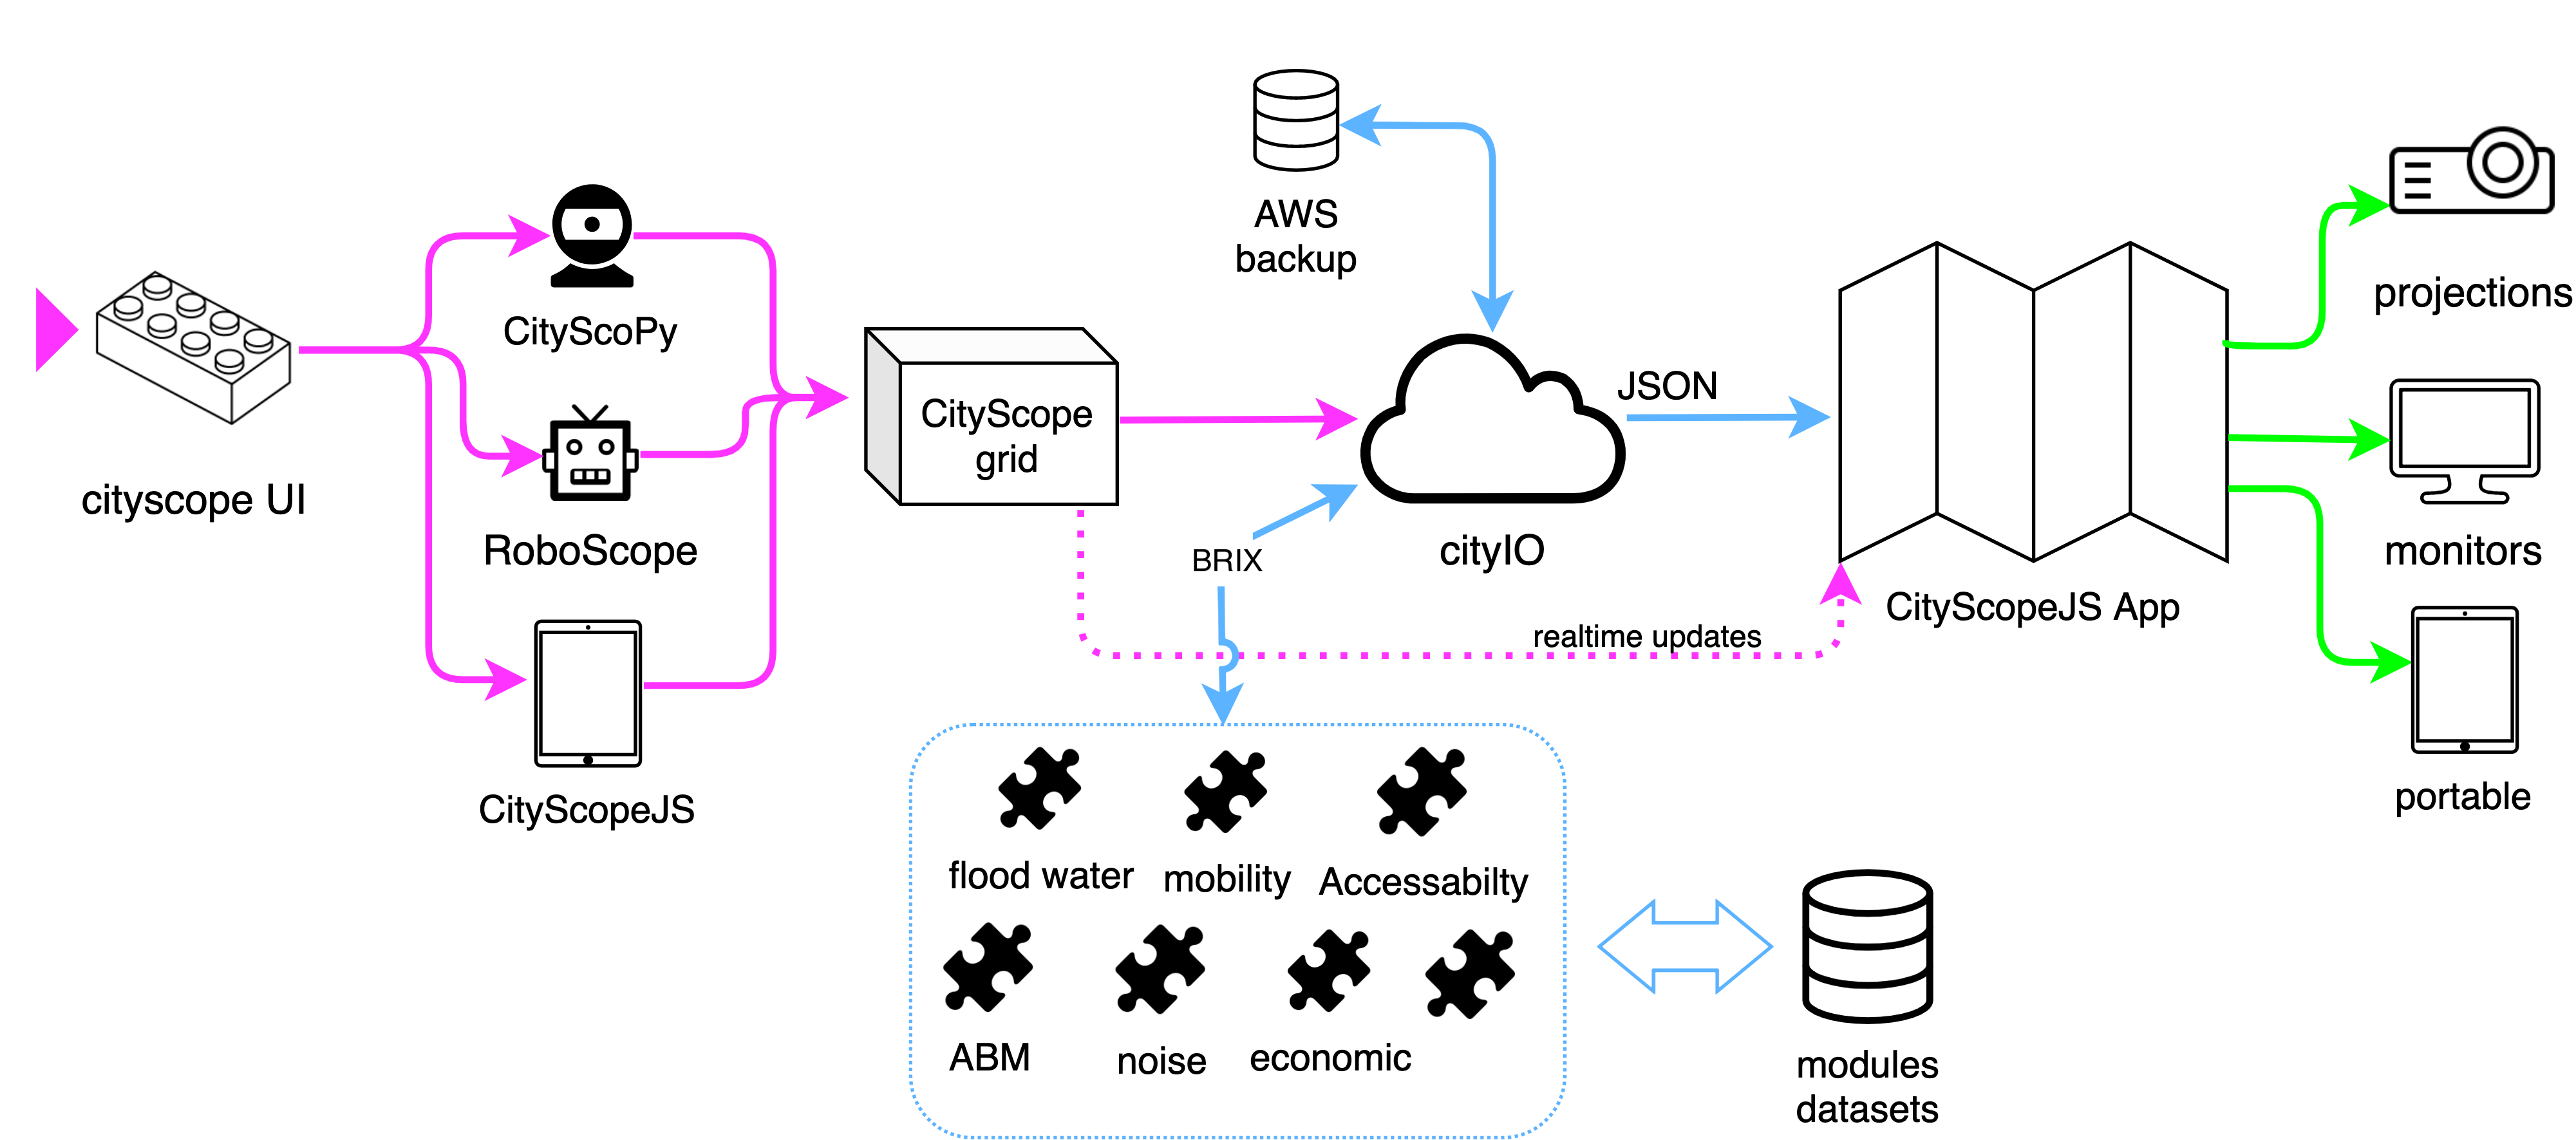
\includegraphics[width=1\textwidth]{chapters/transformation/cs_arch/figures/arch/cs_arch0.png}
      \end{center}
      \caption{
          CityScope Architecture. This diagram presents the data flow and different components of the CityScope architecture: (purple) Different modules control the inputs and CityScope Grid interaction; (blue) Upon interaction, cityIO VPC handles the transaction with different analytics modules; (green) When the computation phase is completed, the grid and analysis modules results are sent to output devices, either online (CityScopeJS, API), or onsite (projectors, monitors)
      }
      \label{fig:cs_arch}
  \end{figure}

  \subsection{Schema and Types System}\label{subsec:types_system}
  {

      \begin{figure}[!htb]
          \begin{center}
              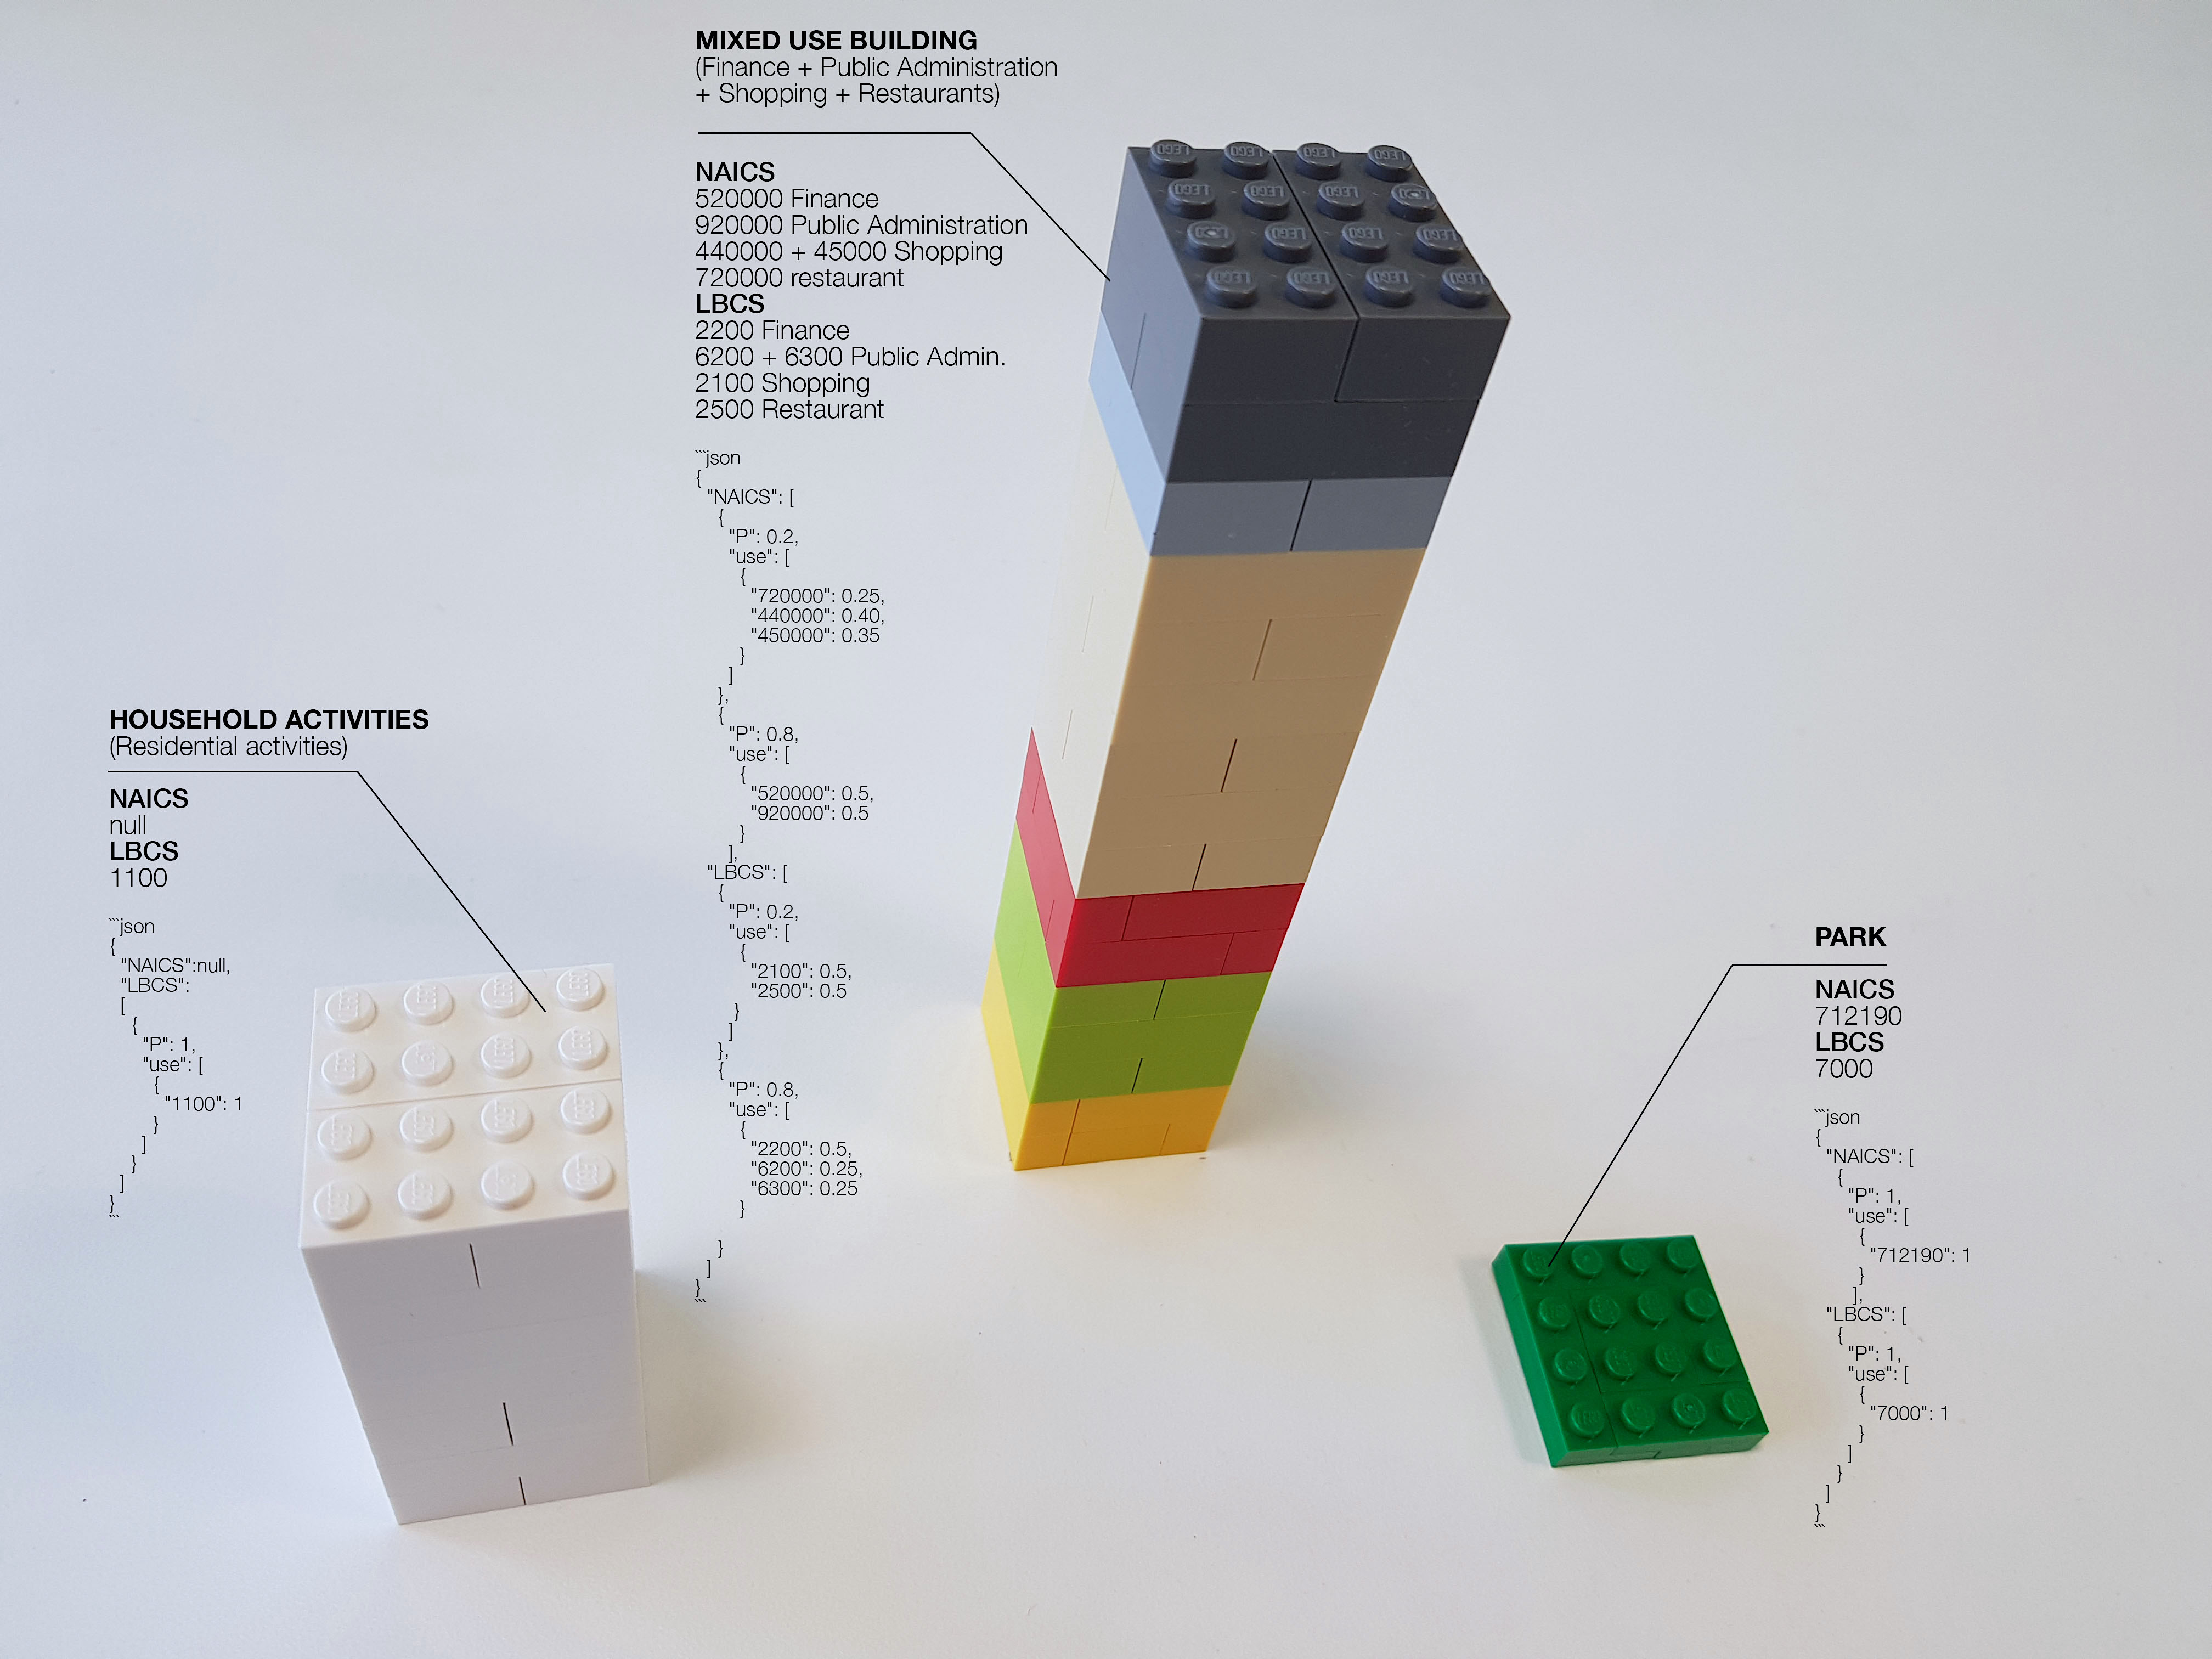
\includegraphics[width=0.8\textwidth]{chapters/transformation/cs_arch/figures/arch/cs_arch1.jpg}
          \end{center}
          \caption{Type System and CityScope Schema. This diagram presents three examples of basic and more complex types as CityScope grid tiles, and how they are encoded in the Schema using LBCS and NAICS codes. (Figure: Luis Alonso, MIT)}
          \label{fig:type_sys_schema}
      \end{figure}

      The CityScope Schema defines a set of \textit{`types'} that are used to describe land-uses, urban functions, and purpose of fixed-size, rectangular geographical-units. These units can then be combined and arranged to represent complex urban environments over a CityScope intervention area, or the  \textit{`grid'}. Types are assigned to all cells in the grid, providing unified segmentation, scale, and a level of abstraction, that can be easily manipulated by users in both physical TUI and virtual interfaces. Cells within the grid can either be immutable or amendable, depending on the project specifications; At minimum, each tile must include one LBCS land-use, but most modules would require also one economic activity. The land-use data is based on the LBCS land-use classification system \cite{montenegro2012land}, and the economic activity data is based on the NAICS codes \cite{NorthAme86:online}\footnote{
          \textit{Land Use Classification Notation} or LBCS classification system includes activity, function, building type, site development character, and ownership constraints in each of its dimensions (for LBCS scheme breakdown, see \eqref{appendix:schema-description}).
          \newline
          \textit{Economic Activity Classification Notation} or NAICS are a standard used by Federal statistical agencies in classifying business establishments for the purpose of collecting, analyzing, and publishing statistical data related to the U.S. business economy. Codes are generated using a numerical classification outlined in the NAICS manual \cite{NorthAme86:online} (for NAICS scheme breakdown, see \eqref{appendix:schema-description}).
      }.
      Types may differ from one project to another, depending on the desired intervention or research question. For example, a CityScope project might include types associated with different levels of energy consumption, in order to asses how certain spatial arrangements can change energy usage.
      \newline
      In order to transfer Schema data between the different components of CityScope, a server system called `cityIO' was designed. The next section details the evolution and design of this system.
  }


  \subsection{cityIO}\label{subsec:csarch-cityio}
  {

      \begin{figure}[!htb]
          \begin{center}
              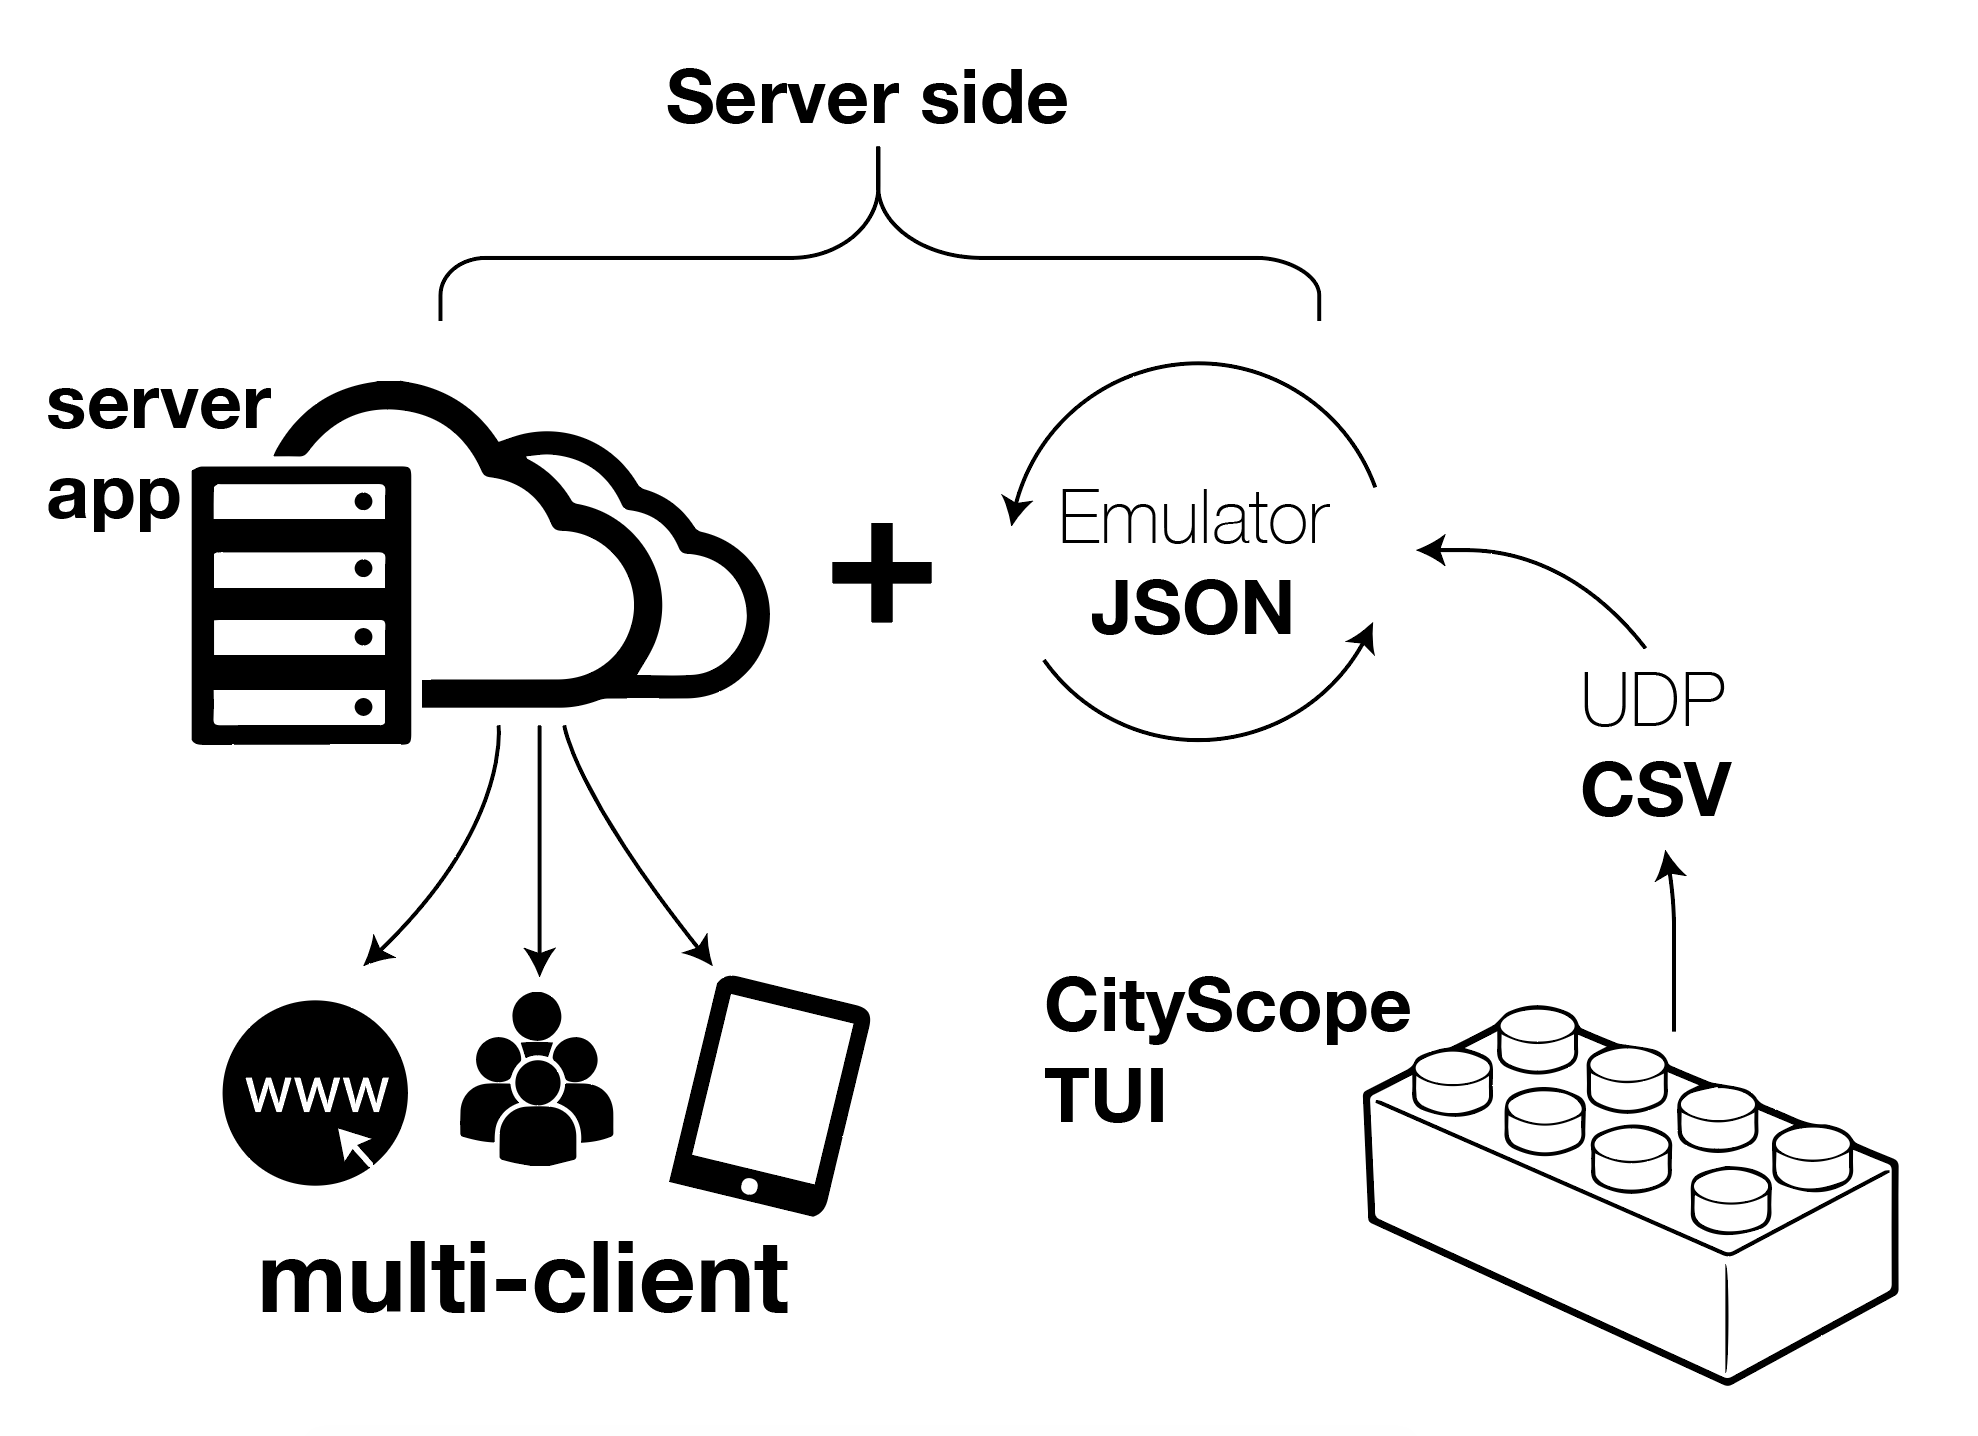
\includegraphics[width=0.5\textwidth]{chapters/transformation/cs_arch/figures/arch/cs_arch2.png}
          \end{center}
          \caption{cityIO V1: Data flow in the early version of cityIO.}
          \label{fig:cityio_v1}
      \end{figure}


      \textit{cityIO} is a CityScope service responsible for the communication between the different components of the CityScope ecosystem. cityIO maintains the current and - in some cases - the past state of CityScope instances, as well as preform other server-side tasks, such as security and user-logging. In 2015, cityIO first version was created with the sole purpose of supporting communication between a tangible user interface (TUI) and a handheld AR device. That version was developed using User Datagram Protocol (UDP), a fast yet unreliable packets-based communication \cite{richard1994tcp}. When users interacted with the CityScope TUI (for example, by moving a LEGO tile), a packet would be sent to the server, and then broadcasted to the AR devices (see Section \eqref{sec:cityscope_ar}). With each interaction, the virtual environment in these devices would react with updated visualizations and analysis. UDP presented several challenges: (i) Its data reliability was limited, and lost data packets caused inconsistent user experience, (ii) UDP was not scalable to web-apps due to security concerns. In 2016, an HTTP server-client system has been proposed to allow more scalable and reliable communication between elements of the CityScope ecosystem.

      \subsubsection{cityIO Ver. 1 (`15-`18)}
      {
          The first version of cityIO was using an HTTP protocol and a REST API, which exposed a simple data packet called \textit{CityScope Grid}. The grid was digital translation of a 2D array of objects, which represented the state of the CityScope TUI; With each user interaction, the grid would update, and sent to the server. The server then stored the grid, so that other microservices or devices could access it. By design, cityIO did not limit the access and modification of the grid by other microservices or devices, so that its state could be updated from all ends of ecosystem (i.e., analysis services, other TUI, etc.). The Grid was a JSON object which included a list of lists; Each element in the list had two numerical variables: $[type, rotation]$. The `type' is a numeric index of a list of land-uses\footnote{These land uses could be as simple as as `offices', `housing', or `road', or more complicated types, such as `offices for large companies with retail at the bottom two floors'}, and the `rotation' is the rotation of the physical tile (i.e., 0 - facing up, 1 - 90° rotation, etc.). As such, a client reading the grid, would assume that the tile $[t,r]$ at position $[i,j]$ is of type $type_t$ and rotated $rotation_r$. A typical data sample of the grid object is shown in the Appendix \eqref{appendix:cityio_output_format}. This cityIO version was built with in NodeJS, python, and later in GO.
          \newline
          \textbf{Usage:} The HTTP bidirectional communication enabled users to not only obtain the state of the CityScope TUI, but also interact and share their opinion during real-time CityScope design sessions. For example, users could select geo-located spots in the virtual grid (such as buildings, parks or roads) and add textual comment to the designs proposed by other users, done by simply extending the JSON object of that grid-cell (for example, see the AR application in Andorra at Section \eqref{sec:andorra-data-observatory}). This type of communication offered designers, decision-makers, and communities a way to participate in a shared physical-virtual design session.
          \newline
          \textbf{Limitations:} First, the lean data structure of the grid was not easily interpretable by other microservices or end-user devices. Each microservice would have to parse the grid object, based on predefined Knowledge of the way the grid was structured. This created inconsistency when some microservices were parsing the grid differently from others. Second, the TUI responsible to share the grids' state, was often triggered by external events, such as light bursts, or a slight movement of the TUI table. This created a torrent of data packets flooding the server, which was not scalable, and created a bottleneck in slow-moving microservices. These issues were addressed in the next version of cityIO.
      }



      \begin{figure}[!htb]
          \begin{center}
              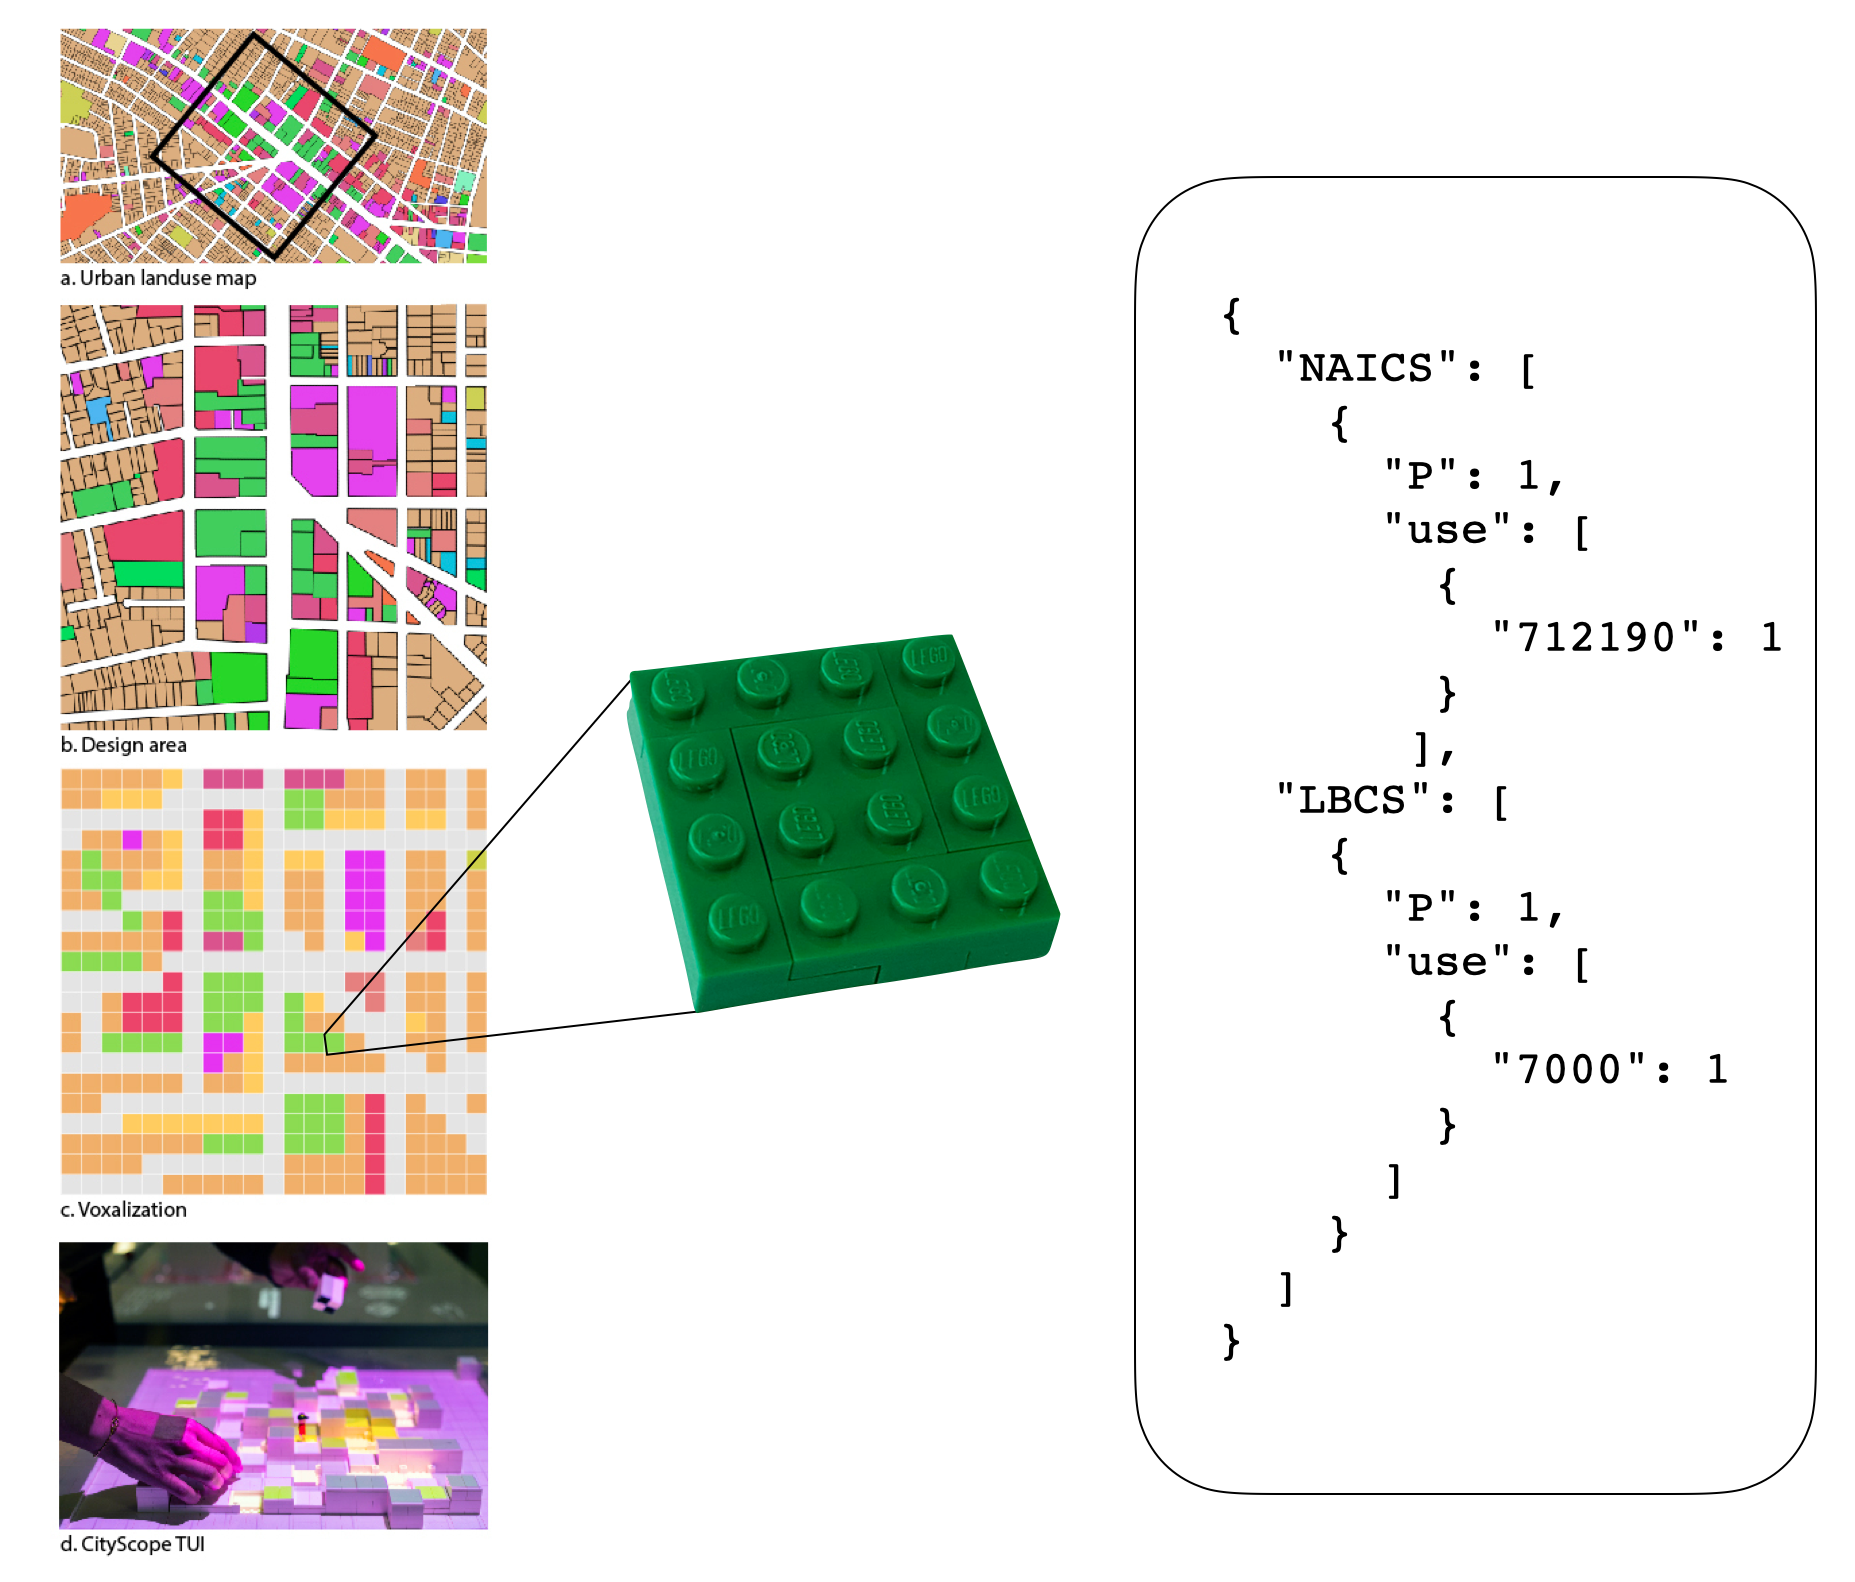
\includegraphics[width=.65\textwidth]{chapters/transformation/cs_arch/figures/arch/cs_arch3.png}
          \end{center}
          \caption{Converting a site to the CityScope Schema: (a,b) designating and aligning an urban intervention site (c) `pixelation' of the site's land-use using the Schema (d) building the TUI for the CityScope context}
          \label{fig:voxel_to_schema}
      \end{figure}


      \subsubsection{cityIO Ver. 2 (`18-current)}
      {
          Amidst these challenges, the second version of cityIO was designed more as a real-time database than a massaging service. The main difference was the implementation of a new CityScope Schema, that was assuming no prior knowledge of the grid, the contextual area, or other baseline information. Instead, the schema was designed as a single JSON object, which hold key-value pairs for the entire data needed for a microserviced CityScope instance. The bare minimum key-value pair is of one \verb|GEOJSON| object called \verb|GEOGRID|, which included all necessary information to render the grid, including geo-location of each grid-cell, their types, and other properties (see examples ver.2 in Appendix \eqref{appendix:cityio_output_format}). Using this object, CityScope users, clients, and microservices could understand the structure of the grid, and parse it in a user-friendly way.
          \newline
          Unlike the first version of cityIO schema, \verb|GEOGRID| is an immutable object, which should not be changed by other microservices. Instead, a mutable object called \verb|GEOGRIDDATA| was introduced, in which only the core properties of each grid-cell are stored. This object is smaller than \verb|GEOGRID|, and is constantly updated by the TUI or other microservices, as needed. The logic behind this design is to maintain a single source of truth for the grid with \verb|GEOGRID|, thus always preserving the initial `tabula-rasa' state of the site in question.
          \newline
          Additional key-value pairs in the root of the CityScope Schema are defined as `CityScope Modules' (see Section \eqref{subsec:cs-modules}), which are the aggregated analysis results of different computational modules or microservices. The next section describes how CityScope modules analyze and evaluate the grid data, and share their results with cityIO.
      }
  }

  \subsection{Microservices and Modules}\label{subsec:cs-modules}
  {
      As discussed in Section \eqref{sec:cityscope_architecture}, CityScope architecture is based on \textit{microservices}, which are a set of computer services that are designed to run independently of each other. The microservices are designed on different platforms and operating systems, so that each service can operate on its designated environment \cite{balalaie2016microservices}. This architecture stems from the idea that each microservice can be designed independently, as long as a shared terminology exist.

      \subsection{Microservices}
      {
          In the context of city-planning and spatial analysis, the CityScope ecosystem requires a wide spectrum of microservices; From straightforward calculations of square footage, to complex noise, energy, or traffic simulations. If in early stages, CityScope was composed of a single service for a single instance (such as the zoning simulation in CityScope Playground, see Section \eqref{sec:cityscope_playground}), the microservices design would allow for each CityScope to preform multiple tasks and analyze various aspects in concurrency.
          \newline
          Another motivation for the development of a microservices architecture, is the need to support the extension of CityScope interfaces beyond the TUI. Decoupling UI, feedback, and analysis microservices allows to add new interfaces, modules, and visualization aids without having to update the existing hardware or software. For example, projects like CityScope Corktown can be fully accessed on a web-browser, where CityScope Ho Chi Minh City would utilize a physical interface, all the while running the same underlying microservice architecture.
          \newline
          Lastly, the microservices architecture is designed to be easily extensible. Since a major aspect of CityScope is open-source and collaborative development, contributions to either frontend, backend, or individual microservices is made possible using detached components. In that manner, the teams working on CityScope Grasbrook (see Section \eqref{sec:grasbrook}) were able to extend the CityScope ecosystem to include new microservices, add functionality to existing ones, as well as redesign the frontend and TUI components as needed.
      }


      \begin{figure}[!htb]
          \begin{center}
              \includegraphics[width=1\textwidth]{chapters/transformation/cs_arch/figures/csjs/csjs_0.png}
          \end{center}
          \caption{CityScopeJS interface. Similar to the TUI versions of CityScope, users interaction is design to be simple and intuitive. Interactions are sent to the cityIO analysis modules, and their responses are then displayed spatially as heat-maps, trips, or graphically as charts and data visualizations. (1) CSjs grid design using a `paintbrush' gesture; (2) animated results of mobility analysis module; (3) results of accessability heatmap to employment and other urban attributes; (4) accumulated traffic results and mobility mode for each road segment.}
          \label{fig:csjs}
      \end{figure}



      \subsection{Modules}
      {
          CityScope Modules is a collection of backend microservices which preform the analysis for a CityScope project. Every time a user interacts with the CityScope interface (via virtual or physical UI), their \verb|GEOGRIDDATA| state is updated on the cityIO server; Modules are constantly listening to these changes, and are triggered to preform analysis with each change.
          When a CityScope module completes an analysis, its results are sent back to cityIO, so that the frontend, and other modules, would have access to it. The analysis results are called `indicators', which can be any of numeric, heatmap, simulation, or textual representation. Numeric indicators are usually displayed as a chart (bar, radar, etc. See Section \eqref{sec:cityscope_volpe}). Heatmap indicators are geo-located (points, lines, or polygons) which are displayed as layers directly on the CityScope table. Simulations are also displayed on the table but are the result of a temporal analysis (such as ABM, mobility simulation, etc) and are therefore displayed as a dynamic layer.
          \newline
          Some modules' results are not directly visualized on the CityScope interface. Instead, these modules would only compute so that other modules could use their results, as part of their analysis. For example, a CityScope table dedicated to the analysis of noise in a new development site, would use mobility simulation to indicate the types and volume of vehicles traversing through the area. The results of this mobility module would not be used for visualization, but instead would become available for the noise module itself. This structure allows greater complexity and dependency of analysis modules. To ensure all modules are synced with the current state of the \verb|GEOGRIDDATA|, cityIO produces a unique hash for each grid state (see Appendix \eqref{appendix:cityio_output_format}). The next section describes how modules' results and user interaction are combined in the CityScopeJS frontend.
      }
  }



  \begin{figure}[!htb]
      \begin{center}
          \includegraphics[width=1\textwidth]{chapters/transformation/cs_arch/figures/csjs/csjs_1.png}
      \end{center}
      \caption{CityScopeJS usage in tangible interfaces. (left) CSjs for the Grasbrook project in Hamburg \eqref{sec:grasbrook}; (right) an early version of CSjs for a student workshop in Aalto University, Espoo, Finland.}
      \label{fig:csjs_tui}
  \end{figure}

  \subsection{CityScopeJS (`CSjs')}
  {
      CityScopeJS\footnote{stands for CityScope Javascript or `CSjs' in short.} is the unified online frontend for the CityScope ecosystem. CSjs is designed to combine the most common use-cases for any CityScope instance: initiation, interaction, visualization, and feedback. CSjs allow users to examine different urban-design alternatives and understand their impact, through a range of KPIs, metrics, visualizations, and charts. It can be used as a standalone online tool, or in combination with TUI in an physical setting. Using its interface, users can edit a grid and change land-uses, buildings, open spaces or transport routes, as well as amend their properties and attributes. As soon as the user concludes their design session, their grid state is sent to cityIO for calculations by the modules. When these are computed, CSjs pulls the new analysis results from cityIO, and displays them on the interface. CSjs is built with ReactJS and DeckGL \cite{ReactAJ49:online,deckgl17:online}. The rest of this section describes the features of CSjs.

      \begin{figure}[!htb]
          \begin{center}
              \includegraphics[width=1\textwidth]{chapters/transformation/cs_arch/figures/csjs/csjs_2.png}
          \end{center}
          \caption{CityScopeJS case-studies. (top-left) CSjs for the CityScope Grasbrook project in Hamburg, 2019 \eqref{sec:grasbrook}; (top-right) CSjs for the Corktown project in Detroit, MI, 2020; (bottom-left) CSjs for the CityScope MoCho, 2018 \eqref{sec:cityscope-mocho}; (bottom-right) CSjs for the Ho Chi Minh City project in Vietnam, 2021.}
          \label{fig:csjs_versions}
      \end{figure}


      \subsubsection{CSjs Features}
      {
          CSjs exposes three main features: \textit{Grid Editor}, \textit{Playground}, and \textit{Projection}. The CSjs Grid Editor is a helper tool to initialize and bootstrap new CityScope projects. It allows the creation of (i) a CityScope endpoint on cityIO (with a dedicated URI); (ii) a virtual, geo-located, 3D, and editable CityScope grid; and (iii) a list of `types' to be used in the design of this CityScope instance. The definition of types and their attributes strictly follows the aforementioned CityScope Schema (see Subsection \eqref{subsec:types_system}).
          \newline
          The \textit{CSjs Playground} is where users interact with the predefined CityScope grid. The interface is built to allow for simple, intuitive, and real-time intervention with the grid setup and land-uses, mimicking the ease of use of a traditional LEGO TUI. Unlike other CAD and planning tools, CSjs interface features minimal functions, toolbars, or menus, and is designed to be used with simple hand gestures on various devices, from an 9 ft TUI table, to a handheld cellphone.
          \newline
          Lastly, the \textit{CSjs Projection} is a tool to visualize the results of the CityScope modules on a TUI interface, such as a tangible grid. This is a passive presentation tool, that listens and renders updates directly from cityIO, without user interaction. This tool uses non-affine projection mapping (homography algorithm) that is designed to render the CityScope Grid and modules results on a physical interface using projectors.
      }

      \subsubsection{CSjs Case Studies}
      {
          CSjs development became a standalone effort in 2019, but was preceded by several projects and experiments since 2017\footnote{Such as CityScope MoCho, see Section \eqref{sec:mocho_api}}. The goal of these was to test the feasibility of web-based CityScope instances. With the increased power of web-based rendering, GPU acceleration, and faster computation, it became clear that many aspects of the CityScope ecosystem could be migrated to the web.
          \newline
          The development of CSjs was boosted by the CityScope Grasbrook project, which presented a real-world use-case for an online, distributed, and collaborative urban-design tool (see Section \eqref{sec:grasbrook}). since 2017, the majority of CityScope projects were built on top of CSjs, such as the Grasbrook, Corktown, EPA, Ho Chi Minh City, Guadalajara, and others. In some cases, developers built their own custom modules, frontend components, or connected CSjs to other TUI. For example, the RoboScope\footnote{see \url{https://www.media.mit.edu/projects/roboscope/overview/}}, an actuated TUI inspired by the MIT Tangible Media inFORM table \cite{follmer2013inform}, uses CSjs to link its TUI to the rest of the CityScope ecosystem. The next subsection describes how other TUI and interfaces are integrated in CityScope.
      }
  }

  \begin{figure}[!htb]
      \begin{center}
          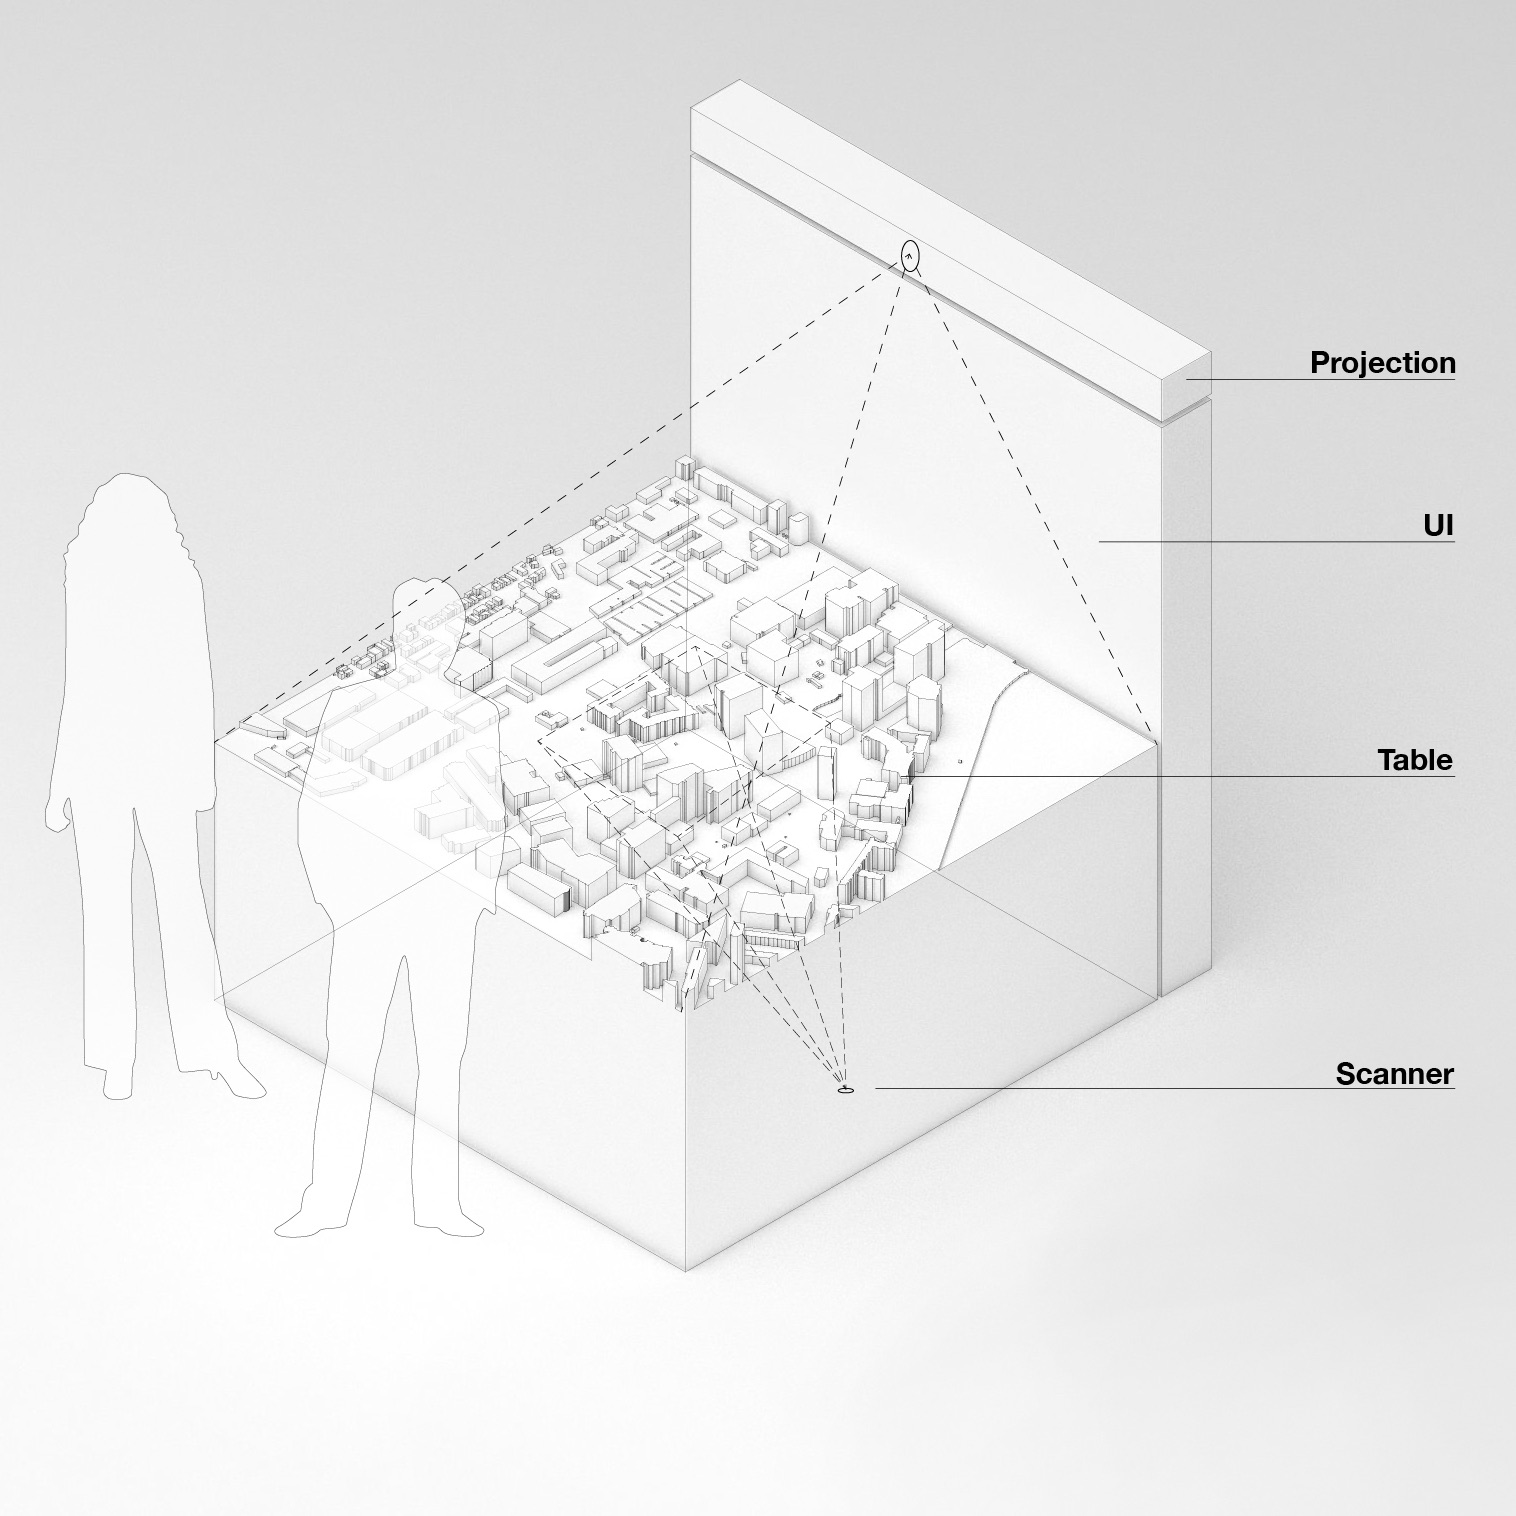
\includegraphics[width=1\textwidth]{chapters/transformation/cs_arch/figures/cspy/cspy_0.jpeg}
      \end{center}
      \caption{CityScope TUI. Physical 3D urban models, scanning module, feedback monitors and projection scheme. Variations of this setup were used in many CityScope projects.}
      \label{fig:cspy_tui}
  \end{figure}

  \subsection{CityScoPy}\label{subsec:csarch-cityscopy}
  {
      CityScoPy is a TUI library for CityScope written in Python. It is designed to recognize interactions with physical objects equally distributed over a 2D grid (such as LEGO tiles), and send the scanning results as a JSON object to cityIO (see Appendix \eqref{appendix:cityio_output_format}, \eqref{appendix:cityscopymethods}). CityScoPy exposes several functionalities, such as keystoning, scanning, and sending data to different endpoints, as part of the microservices architecture of CityScope. CityScoPy is built in Python and OpenCV for image processing \cite{opencv_library}.


      \begin{figure}[!htb]
          \begin{center}
              \includegraphics[width=1\textwidth]{chapters/transformation/cs_arch/figures/cspy/cspy_2.png}
          \end{center}
          \caption{CityScoPy scanner in action. This version of CityScoPy was created in vanilla Javascript to run on low-tier devices, such as cellphones or Raspberry-Pi with a basic web browser. Later versions were written in Python for faster scanning of larger grids.}
          \label{fig:cspy_scan_in_action}
      \end{figure}

      \subsubsection{Background}
      {
          CityScoPy is part of a long line of scanning tools developed over the years to support TUI for spatial analysis. Sensing the location of physical objects on a tabletop was prototyped in the exhibition ``Unbuilt Ruins''\footnote{By Kent Larson, displayed in Penn Architecture Archives (1999) and at `The Un-Private House' in the MOMA, NYC (1999)}, which featured digital-physical objects poised on top of a Louis Kahn's building blueprint \cite{sparacino1999technologies}. As users repositioned the objects, an array of projectors reviled rendered images associated with that object's location. Similar ideas were developed in the SandScape table \cite{ishii2004bringing}, where a digital relief of physical objects was captured in real-time using a top-down scanner. Since 2013, several scanning methods were developed by the CityScope team to capture physical objects and use them to simulate intervention and perform urban analysis \cite{Hadhrawi2016, zhang2017citymatrix, aldawood2014interaction}. These tools all shared the idea of scanning an array of predefined set of objects from beneath a translucent tabletop. The objects types were differentiated using colorful LEGO pieces, and the scanner was designed to recognize the objects' type and locations as users interact with them.
      }
      \subsubsection{Motivation and Design}
      {
          \begin{figure}[!htb]
              \begin{center}
                  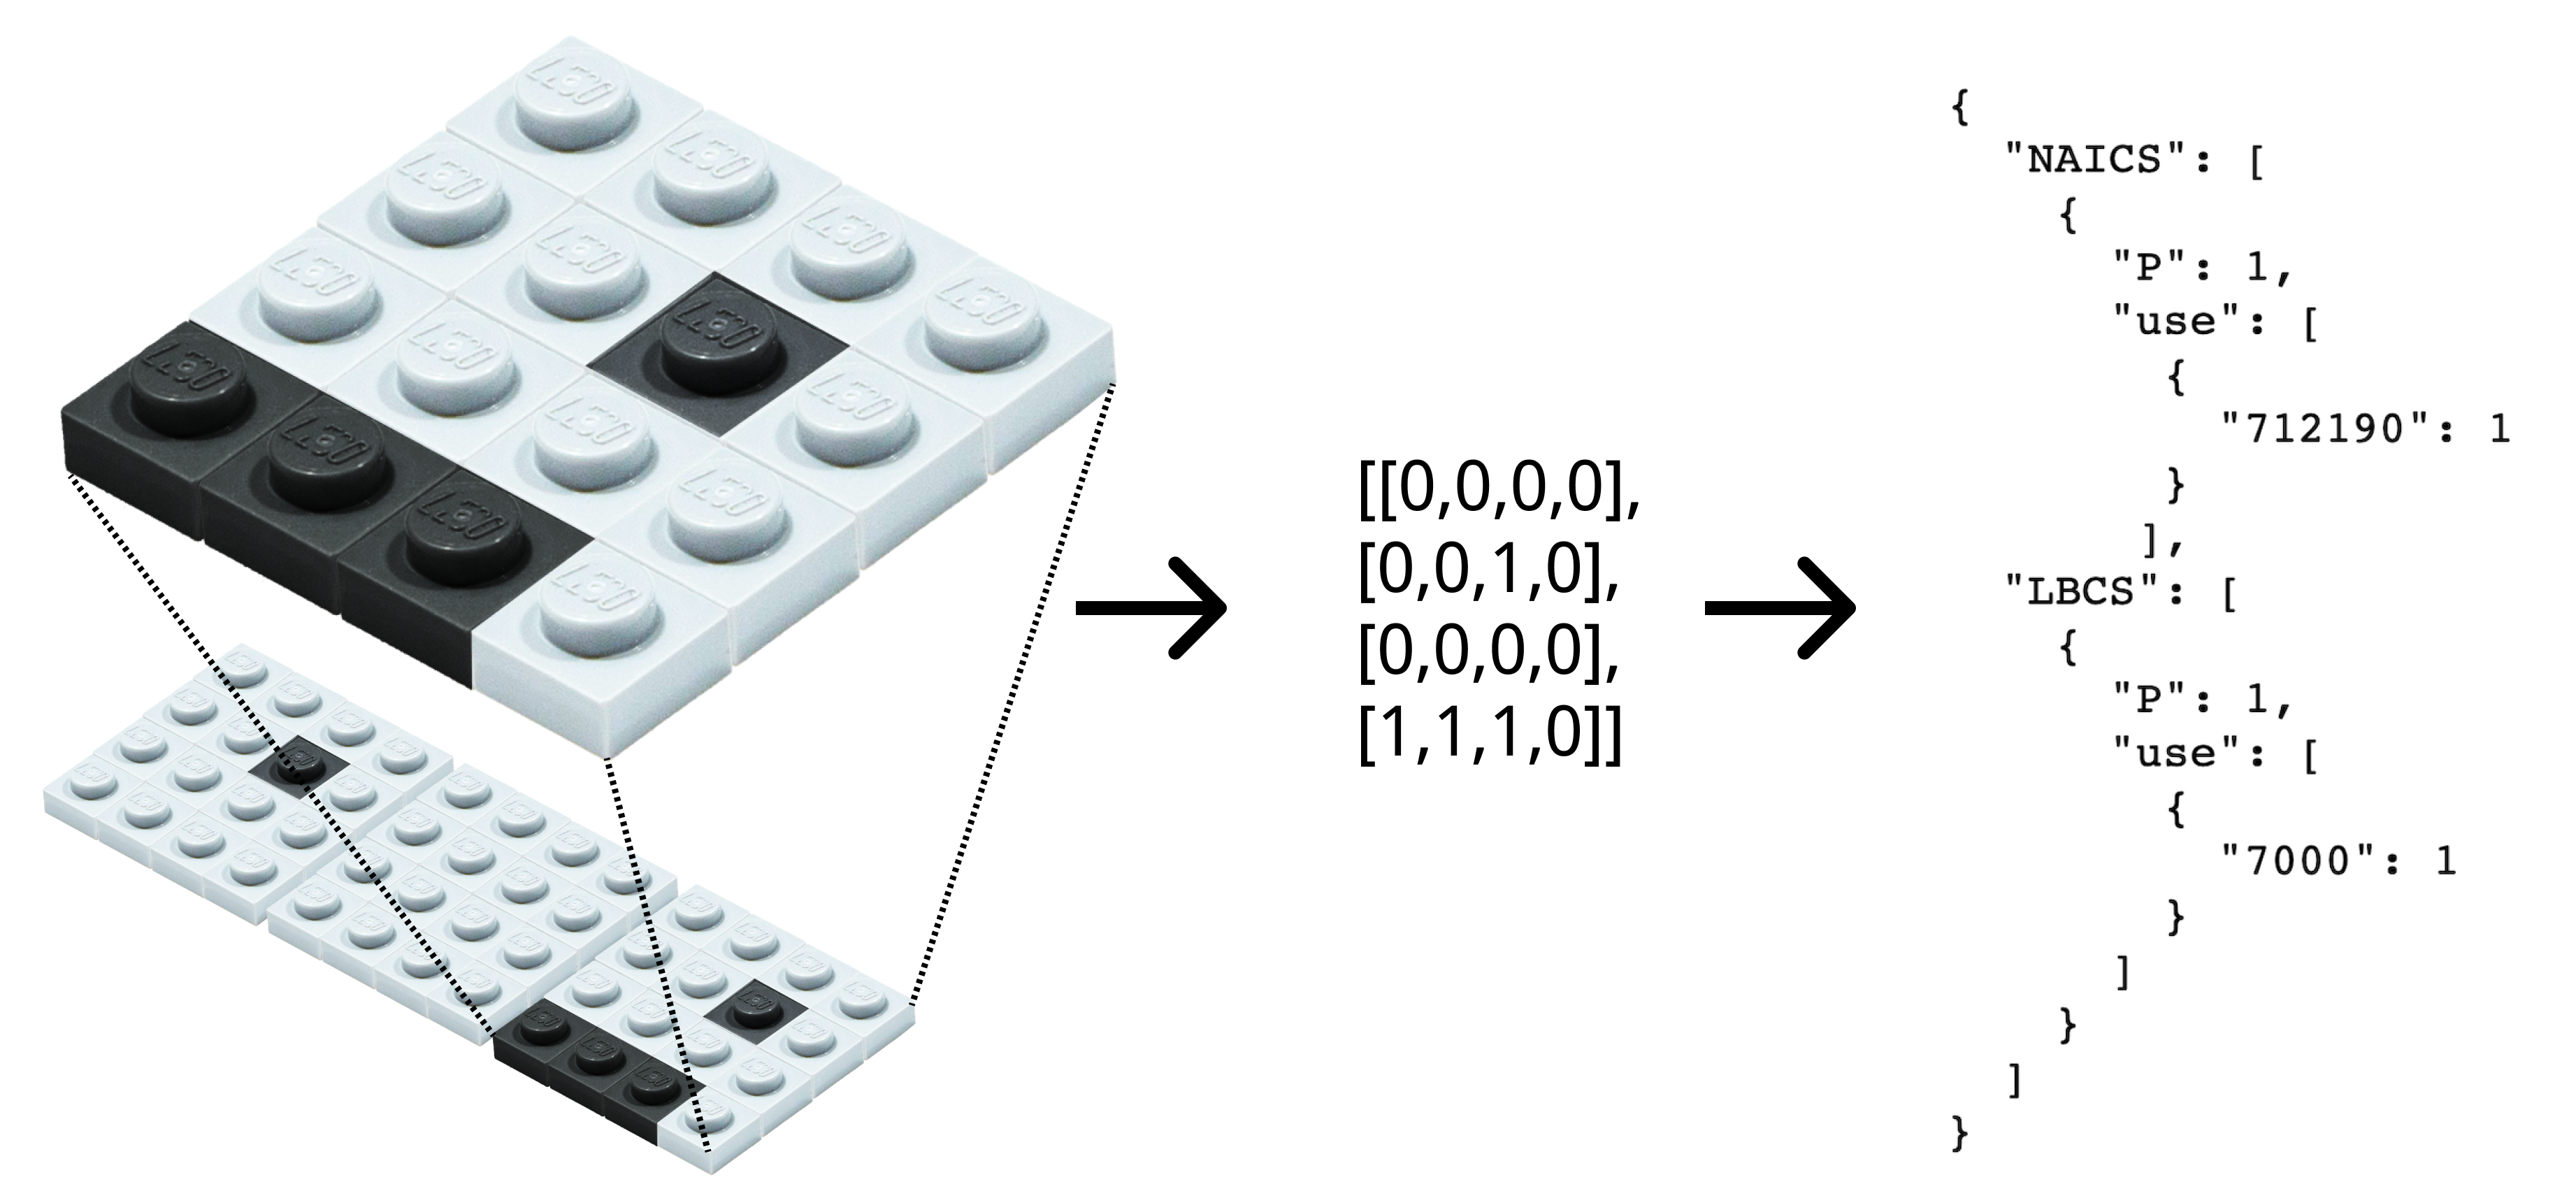
\includegraphics[width=1\textwidth]{chapters/transformation/cs_arch/figures/cspy/cspy_3.png}
              \end{center}
              \caption{Example of a CityScoPy scanning result. The grid is scanned for binary values, and a 2D matrix is created to represent the grid cell. For each cell, a key-value pair search is conducted to find the corresponding type in the CityScope Schema.}
              \label{fig:cspy_results}
          \end{figure}

          CityScoPy was developed in order to improve several shortcomings in previous CityScope scanners: (i) \textit{Speed:} CityScoPy was designed to handle larger and more complex CityScope grids than before (see \eqref{subsec:vople_cityscope})\footnote{When tested on a 2015 Macbook Pro, CityScoPy scanned a grid of 100x100 4x4 LEGO tiles (total of 160000 scanned items) at 40fps.}. (ii) \textit{Versatility:} CityScoPy introduced a simple binary code, in which each of the LEGO studs of a 4x4 tile would be considered as either white or black\footnote{For example, a pattern with 4 white dots in the top-left corner and black in the rest would be [1,1,0,0,1,1,0,0,0,0,0,0,0,0,0,0].}. Using hues at the edges of the color gamut simplified the scanning algorithm, while still yielding $2^{16} = 65536$ unique permutations. This offered greater flexibility than the previous versions, while maintaining a simple way to differentiate types. (iii) \textit{Stability:} Previous CityScope scanners used a combination of colorful objects to identify types. These were proven unstable, since the scanner would tend to observe the same color at different parts of the tabletop as different RGB values. Since CityScoPy uses a binary code to define each type, the possibility of errors are reduced to the edge cases in the center of a gray-scale gamut. Additionally, the scanning algorithm captures and averages an array of 10x10 pixels for each scanning point, in order to reduce the potential of a faulty reading due to hazing or light bursts.
      }
      \subsubsection{Use-cases}
      {
          CityScoPy was adapted for several projects in HafenCity University, including the SmartSquare \cite{bley2020smartsquare} and CityScope Grasbrook \cite{baeza2021cityscope}. It was also used in several City Science network labs, such as Shanghai, Aalto, Guadalajara, and Jerusalem. At MIT, it was used for CityScope MoCho \cite{doorley2019s}, DeepScope \cite{noyman2020deepscope}, among others. In 2018, CityScoPy was used as part of an interactive installation for `The Road Ahead: Reimagining Mobility' exhibition in the Cooper-Hewitt Museum of Art, NYC \cite{CityScop40:online}. This CityScope artistically featured two extreme versions of a future with driverless cars: In one scenario, streets are dominated by vehicles which lead to congestion and anxiety; The other is a more vibrant city, where the benefits of walkability, mixed-use, density, and equity increase. In this context, CityScoPy allowed visitors to playfully interact with a fictional NYC-like urban grid, and impact the density and organization of the urban-scape in these two scenarios.
      }
  }

  \subsection{CityScopeAR}\label{sec:cityscope_ar}
  {
      \subsubsection{Introduction}
      {
          As discussed in Section \eqref{sec:cityscope_architecture}, the CityScope system design allows new ways to interact, visualize, and extend CityScope beyond the limitation of physical objects. CityScopeAR is a mixed-reality interface for CityScope, designed for remote yet collaborative urban-design processes. CityScopeAR builds on prior art using mixed-reality devices for CAD and urban-planning purposes (see Chapter \eqref{chapter:introduction}). The goal of CityScopeAR is to use hand-held devices such as smartphones, tablets, AR glasses, or VR headsets, and create a virtual environment that extends the tangible interface of CityScope, allowing users to interact with both the physical world and its virtual representation.
      }

      \subsubsection{System Design}

      {
          As discussed above in Section \eqref{subsec:csarch-cityscopy}, CityScope TUI tend to include a 3D urban model, projectors, and sensors to detect user interactions. Previous usability studies found several shortcomings in these setups \cite{Noyman2015power, Alrashed2015}: First, CityScope tables use flat-top tangible pieces projected with symbols and colors. In active participatory sessions, tables tend to get obstructed throughout most of the session, thus not communicating information as needed. Second, is the challenge of mixing different layers of information onto a single TUI; In user studies (see Section \eqref{sec:brt}), users requested different data layers to be displayed simultaneously. For example, experts might want to view traffic simulation, while member of the community wish to view the noise analysis layer. Lastly, CityScope TUI had no mechanism to systematically collect, store or display users' input and feedback. As shown in the Boston BRT project \eqref{sec:brt}, traditional surveys were used to collect users' feedback. All these suggested that alongside the CityScope TUI, additional representation and interaction methods should be explored.
      }

      \begin{figure}[!htb]
          \begin{center}
              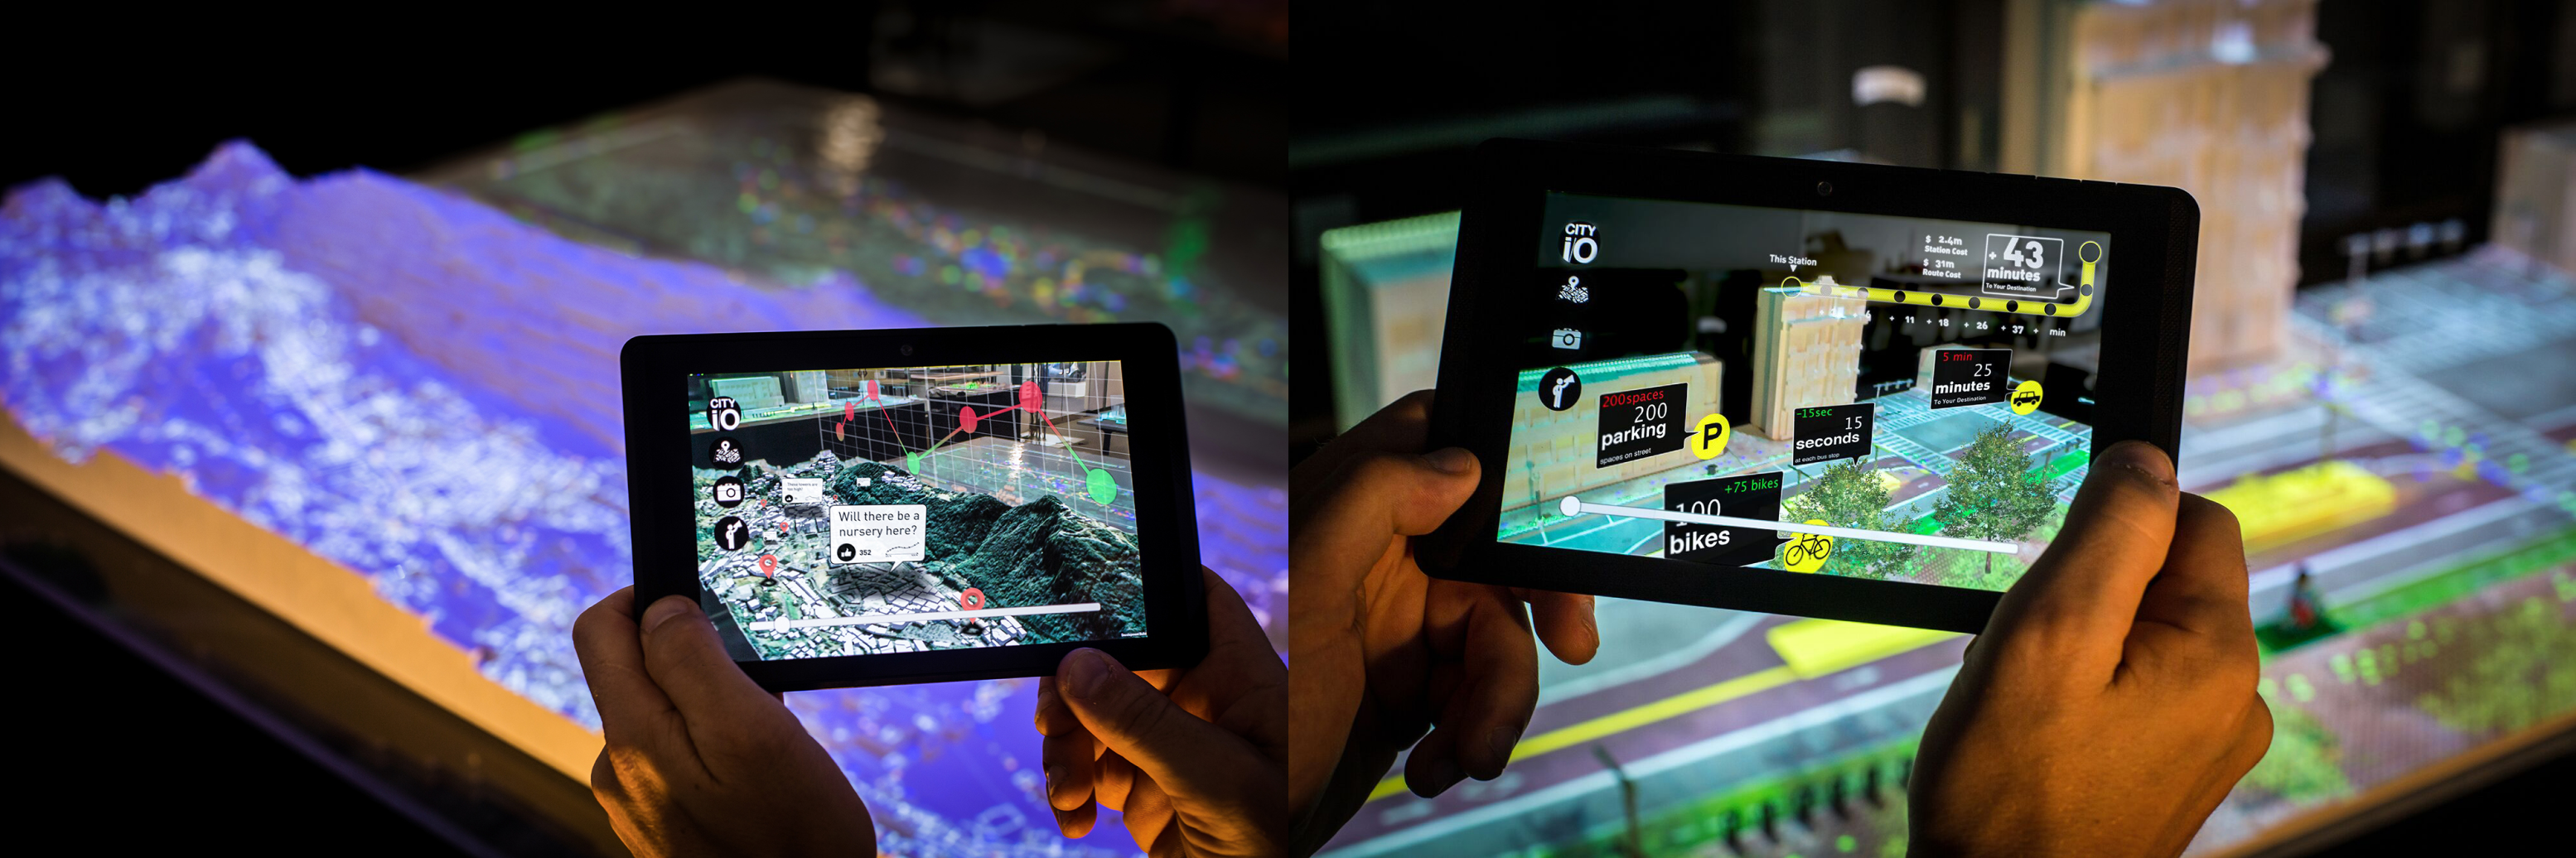
\includegraphics[width=1\textwidth]{chapters/transformation/cs_arch/figures/ar/ar_2.png}
          \end{center}
          \caption{CityScopeAR extends the TUI with additional layers of analytics, data, and public participation. (left) CityScopeAR in Andorra used to collect user input concerning planning and urban development \eqref{sec:andorra-data-observatory}. (right) CityScopeAR for Boston BRT `Street Scale', showing traffic stats and impact on street area in accordance to the different BRT system type \eqref{sec:brt}.}
          \label{fig:csar_two_examples}
      \end{figure}


      \subsubsection{CityScopeAR Prototypes}
      {
          The first iteration of CityScopeAR was prototyped in 2015; A Macbook laptop displayed spatial layers that were mapped to the extents of a CityScope TUI using a set of colorful markers at the edges of the table. These data layers included physical elements (such as 3D building facades, sunlight, shadows, and vegetation), as well urban data layers (such as spatial analysis, heat maps, or interactive points of interest). This tool was developed using Unity and Vuforia SDK \cite{UnityRea35:online}, which were later replaced by Google's ARtoolkit and Nexus 9 tablets. In 2016, development of CityScopeAR shifted to the Google Tango Project; Tango devices allowed better object recognition and preflight area-learning, which was effective in challenging light condition imposed by CityScope projections. However, Tango's low market penetration put this development effort to an end in early 2017 \cite{kastrenakes2017google}. Later, CityScopeAR was developed with Google ARcore and Apple ARkit \cite{oufqir2020arkit}, which are now available on most mobile devices.
      }

      \subsubsection{Tests and Deployments}
      {
          \textbf{BRTCityScopeAR for Boston BRT:} CityScopeAR was developed alongside several key CityScope projects, which offered the opportunity to test and gather feedback on usability and experience. In early 2015, the `Boston BRT' project (see Section \eqref{sec:brt}) included several CityScope TUI which were used in community engagement events. A version of CityScopeAR was designed to augment several data layers: (i) BRT system performance information, such as trip duration, congestion or construction costs; (ii) a mixed-reality layer of BRT station architectural design, signage, building facades and vehicles; and (iii) Agent Based Simulation of pedestrians, cars, bikes, and busses who traversed through the area. Specifically, the simulation was designed to highlight a problem known as `waiting time paradox' \cite{avineri2004cumulative}, which refers to the frustration threshold of public transit commuters. The simulation meant to show how certain BRT design decisions can be made to reduce waiting time and travelers' frustration.


          \begin{figure}[!htb]
              \begin{center}
                  \includegraphics[width=1\textwidth]{chapters/transformation/cs_arch/figures/ar/ar_0.png}
              \end{center}
              \caption{CityScopeAR use-cases. (top-left) Andorra, in the Smart Cities conference, Barcelona \eqref{sec:andorra-data-observatory} ; (top-right) Boston BRT \eqref{sec:brt}; (bottom-left) Real-time interaction analysis with the TUI as a 3D heatmap; (bottom-right) Commenting interface for public engagement.}
              \label{fig:csar_world}
          \end{figure}


          \textbf{AndorrAR:} In 2016, a version of CityScopeAR was developed as part of a research collaboration in Andorra. Nicknamed `AnodrrAR', this variant was deployed at the Smart Cities conference in Barcelona, and later was set on permanent display at the Innovation Space in Caldea, Andorra la-Vella. AnodrrAR was designed as part of an interactive CityScope model which depicted several data layers: (i) Satellite imagery, 3D model of Andorra's landscape and urban areas designated for redevelopment; (ii) cell towers location, and simulation of the population interpreted from CDR data (see \eqref{sec:andorra-data-observatory}); (iii) interactive design proposals for the downtown area, collected from CityScope TUI via cityIO (see Section \eqref{subsec:csarch-cityio}). In this version, users could position and scale master-plans onto geo-located anchors in the virtual city model; and (iv) feedback system, allowing users to comment on urban developments using a virtual `Speech Bubble' interface.
          \newline
          During the Smart Cities conference in Barcelona, hundreds of visitors interacted with the tools, and over 200 feedback comments were recorded during each day of the event. Similar versions of CityScopeAR were deployed in Hamburg at the HCU university (`16), Volpe redevelopment site in Cambridge (`17) and in Shanghai, Tongji University (`17).
      }

      \subsubsection{CityScopeAR: Discussion}
      {
          CityScopeAR extends the CityScope process in terms of scale and location. It retains a linkage to the CityScope tangible interface, while augmenting it with on-demand data, analysis, and feedback. The feedback mechanism added a new layer to the CityScope ecosystem, allowing users to comment on urban development proposals, in a shared virtual or physical design session.
          \newline
          Despite its potential, AR technology is still relatively new, and has yet to reach mainstream usage \cite{mekni2014augmented}. CityScopeAR was an preliminary step towards adoption of AR technology for urban-design, but it also highlighted the challenges of the current state of the art. Specifically, cultivating a collaborative design process using individually hand-held devices was found to be a challenge. A major advantage of the CityScope TUI is in its ability to serve a common ground for conversation and feedback, unobstructed by devices. At the time of writing, even the most advanced AR or VR systems are still struggling with ease of use, accessability, comfort, and performance, hindering their mass use in a collaborative public setting.
      }
  }

  \subsection{Discussion}
  {

      This section discussed the various components of the CityScope ecosystem. It explored the CityScope Schema, a data structure and a standard used across the platform. It detailed the three main components of CityScope: (i) Input and interaction, (ii) urban analysis microservices, and (iii) feedback and visualizations. As a design decision, only few aspects of the CityScope ecosystem are immutable and fixed; Instead, the majority of the ecosystem is designed to be flexible and adaptable to the unique needs of the CityScope community, such as supporting a wide range of urban analytics modules, or the development of different input, visualization, and feedback modalities. The rest of this Chapter shows how this ecosystem was utilized in key CityScope projects.
  }
 }

    %%%%%%%%%%%%%%%%%%%%%%%%%%%%%%%%%%%%%%%%%%%%%%%%%%
    \section{CityScope Playground}\label{sec:cityscope_playground}

{
    \subsection{Introduction}
    {
        In complex decision-making processes, stakeholders from varying backgrounds and expertise are involved. The existing frameworks for city-planning are often designed around certain professional audiences (e.g., planners and architects) and are usually less accessible to a wider scope of users \cite{ben-joseph2001}. A collaborative interactive system could facilitate stakeholder dialogues and interactions, and consequently help them make more informative decisions in shorter time.
        \newline
        This work examines user engagement and decision-making in the context of urban-regulations and zoning. The objectives of this study are twofold: (i) to examine user interactions with tangible user interfaces for urban-planning, and (ii) to investigate stakeholders' engagement and decision-making using these tools.
        This observational study was conducted with a representative sample of users from different backgrounds. These were invited to examine the usability of a CityScope variant developed in 2015, called `Playground'. A comparative analysis of different approaches examined the users' interaction and decision-making using CityScope, in comparison to traditional planning aids. The sessions involved decision-making scenarios using paper-based planning documents, alongside an interactive tangible models of the design area. A coding scheme was developed for analyzing video observations, to examine the wide spectrum of actions, verbal cues, and non-verbal gestures, and quantify the occurrences of these interactions during the experiment.
    }

    \begin{figure}[!htb]
        \begin{center}
            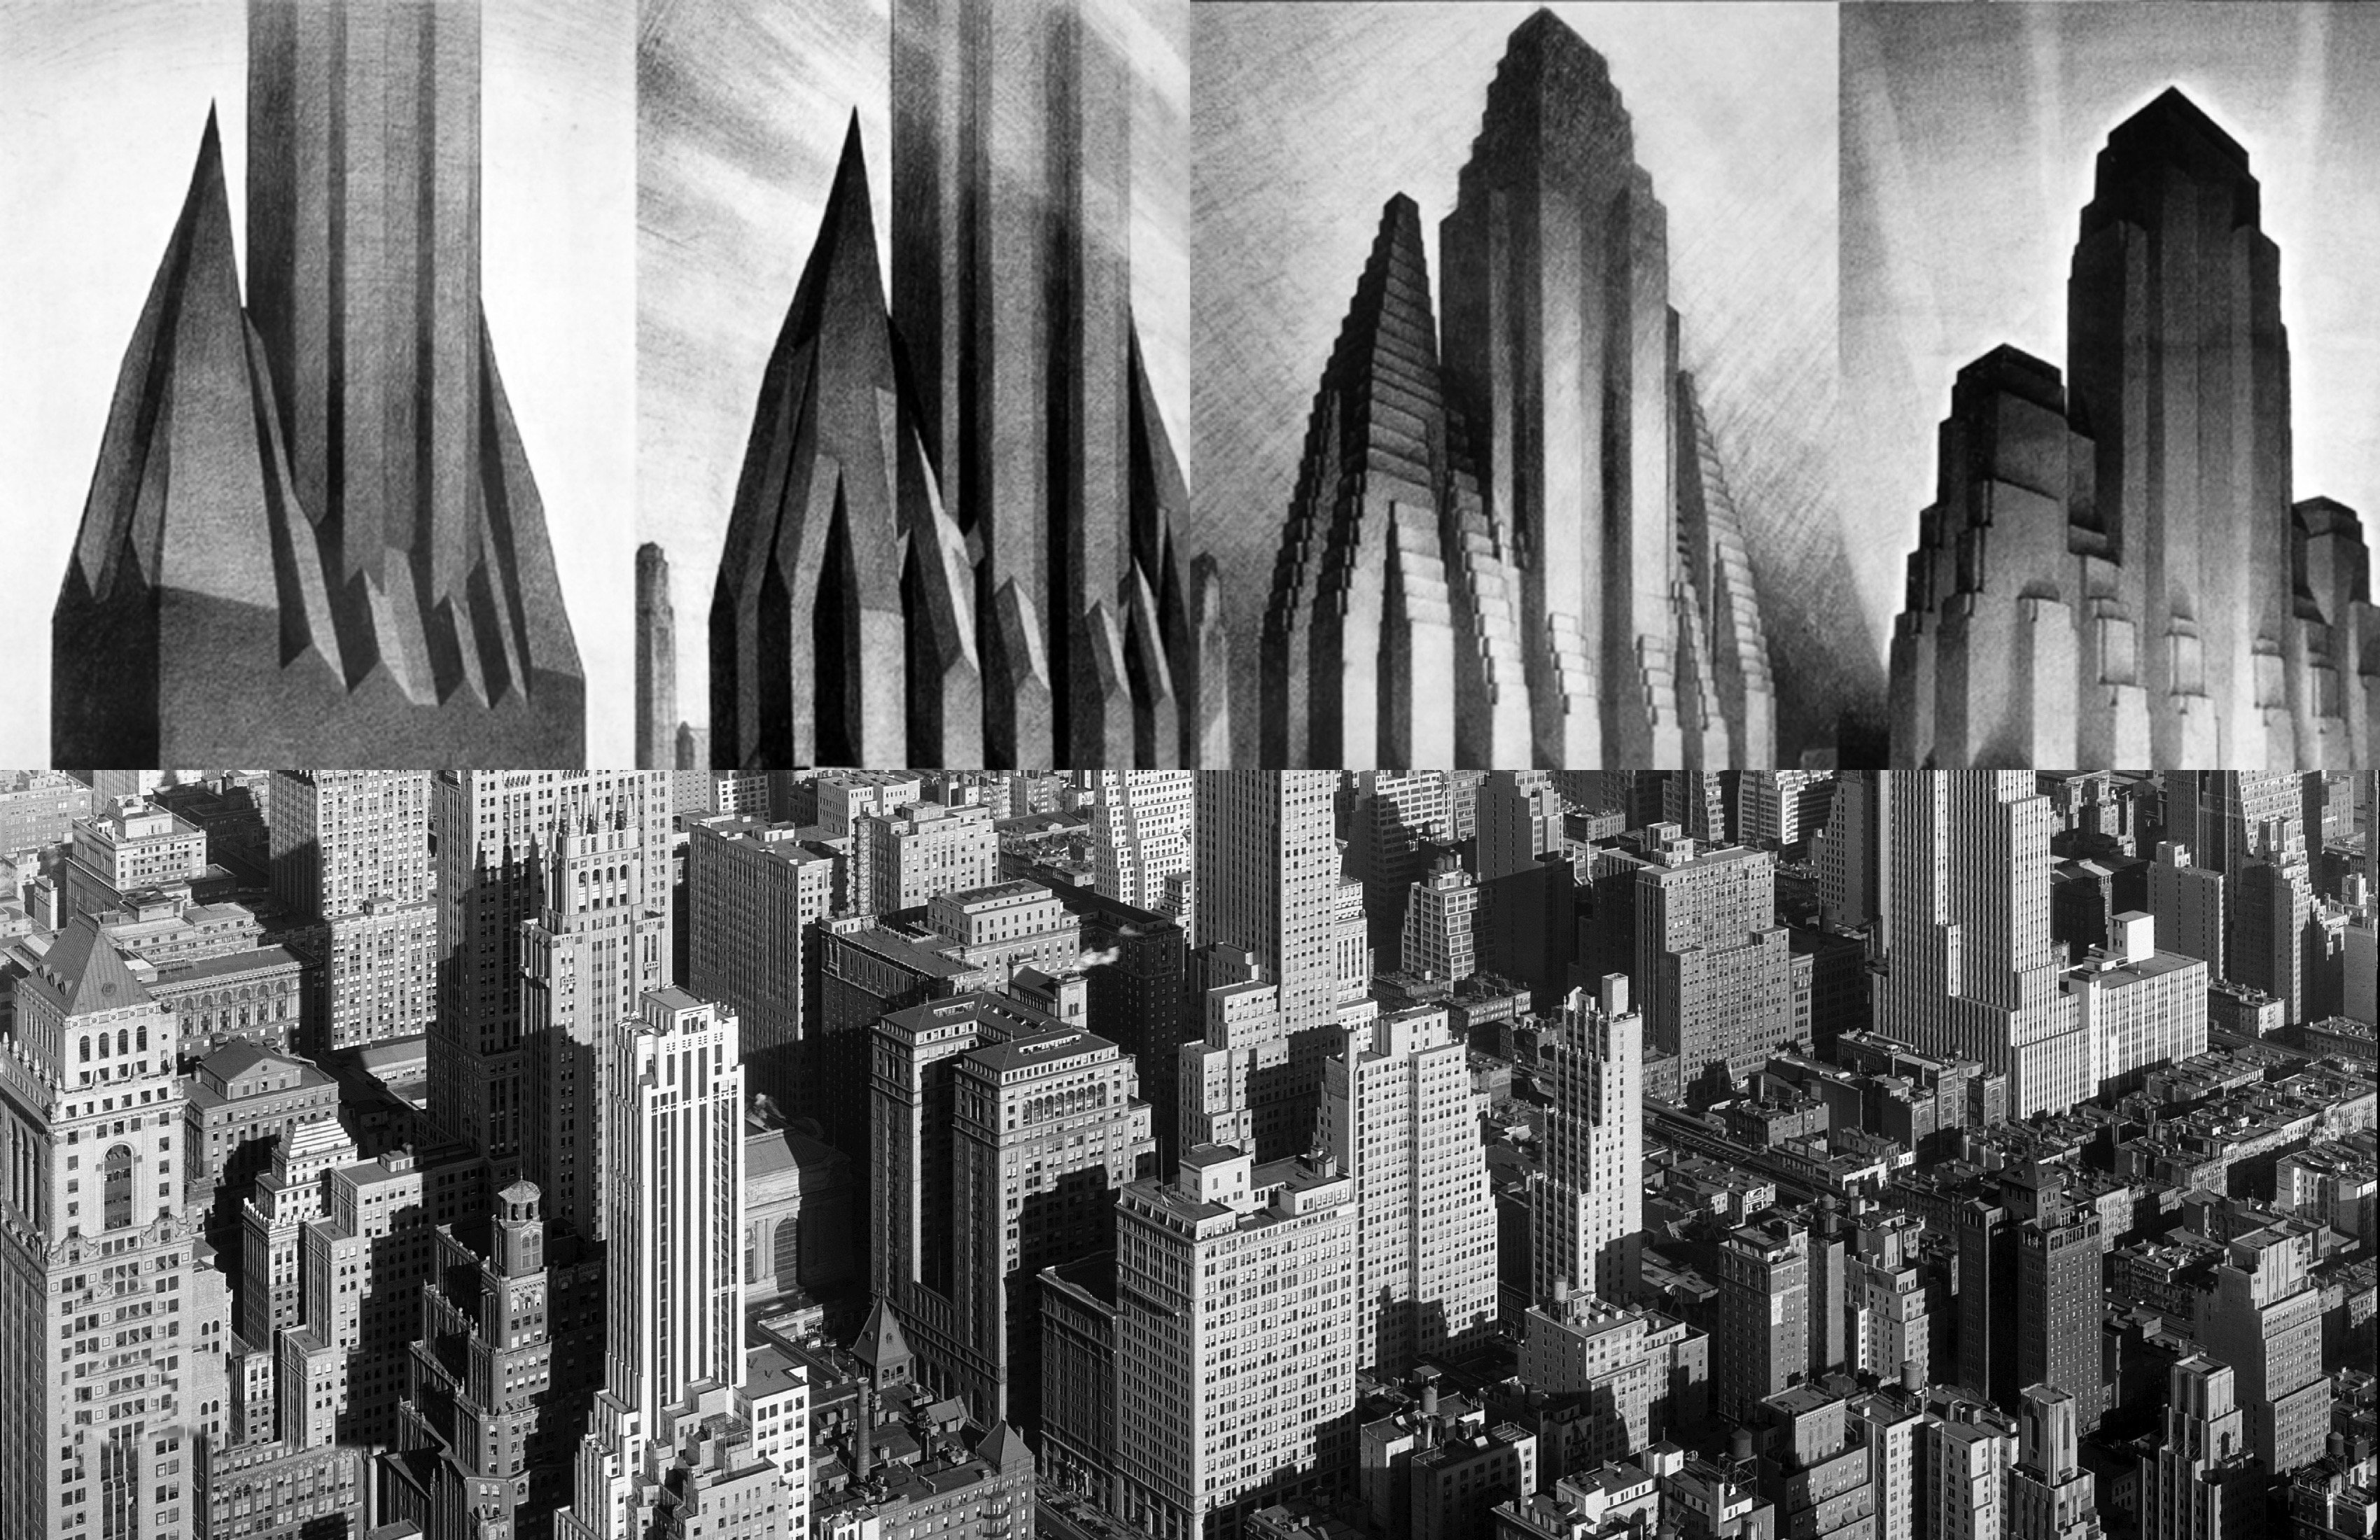
\includegraphics[width=1\textwidth]{chapters/transformation/playground/figures/playground.jpeg}
        \end{center}
        \caption{Impact of zoning-codes and building regulations on urban form. (top) Hugh Ferriss's drawings of NYC 1916 Zoning Ordinance (1922), the first in the United States to regulate building use, floor area, and height of new buildings. (bottom) The effect of zoning on built form and function in Midtown Manhattan.}
        \label{fig:pg_nyc}
    \end{figure}

    \subsubsection{Evaluating UHCI}
    {
        Technologies to support stakeholders in the decision-making process have evolved over the past few decades (see Chapter \eqref{chapter:introduction}). Intuitive tools can create collaborative interaction spaces, where users efficiently work with each other and see the result of their interaction immediately \cite{ishii2002augmented}. Nevertheless, studying the usability and efficiency of such systems is relatively unexplored \cite{Innes2016}.
        \newline
        Several observational studies have been conducted on TUI. Brereton and McGarry \cite{brereton2000observational} tested the usability of tangible objects, and how TUI encourages engineers' design thinking and communication. Fjeld and Sissel \cite{fjeld2002alternative} tested the usability of TUI compared to alternative traditional 3D and 2D single user tools, by examining the learning effect and the overall user experience. These studies showed that 3D tools outperformed in terms of user satisfaction. Falcao and Price \cite{price2009effect} focused on investigating collaborative activities in a tangible table-top environment, to support how shared interfaces affect the way collaborative activities are structured, and examines the kinds of interactions that are productive for learning. Ben-Joseph examined the Luminous Planning Table (LPT) \cite{ben-joseph2001}, in order to further develop its functionality based on feedback from end-users through implementation of an actual parcel slated for development.
        \newline
        This observational study examines the usability of CityScope in a simulated urban-planning process, and investigates its effect on stakeholders' engagement and decision-making. The study aimed to improve the understanding of how a mixture of TUI and virtual environments might encourage collaboration and communication among stakeholders, and lead to better decision making.
    }

    \subsubsection{Kendall Square: Site and Context}
    {
        The study examined user engagement in the context of an early stage city-planning. At this stage, zoning-laws and building-regulations are leading many of the design decisions, and are responsible to the creation of `zoning envelopes': legal frameworks to which the development of new buildings and landscapes is bounded \cite{n15, Ben-Joseph2004}. The preliminary stage of most planning processes is a comprehensive understanding of the spatial and regulatory context. Figure \eqref{fig:pg_nyc} shows the impact of zoning on urban form in NYC.

        \begin{figure}[!htb]
            \begin{center}
                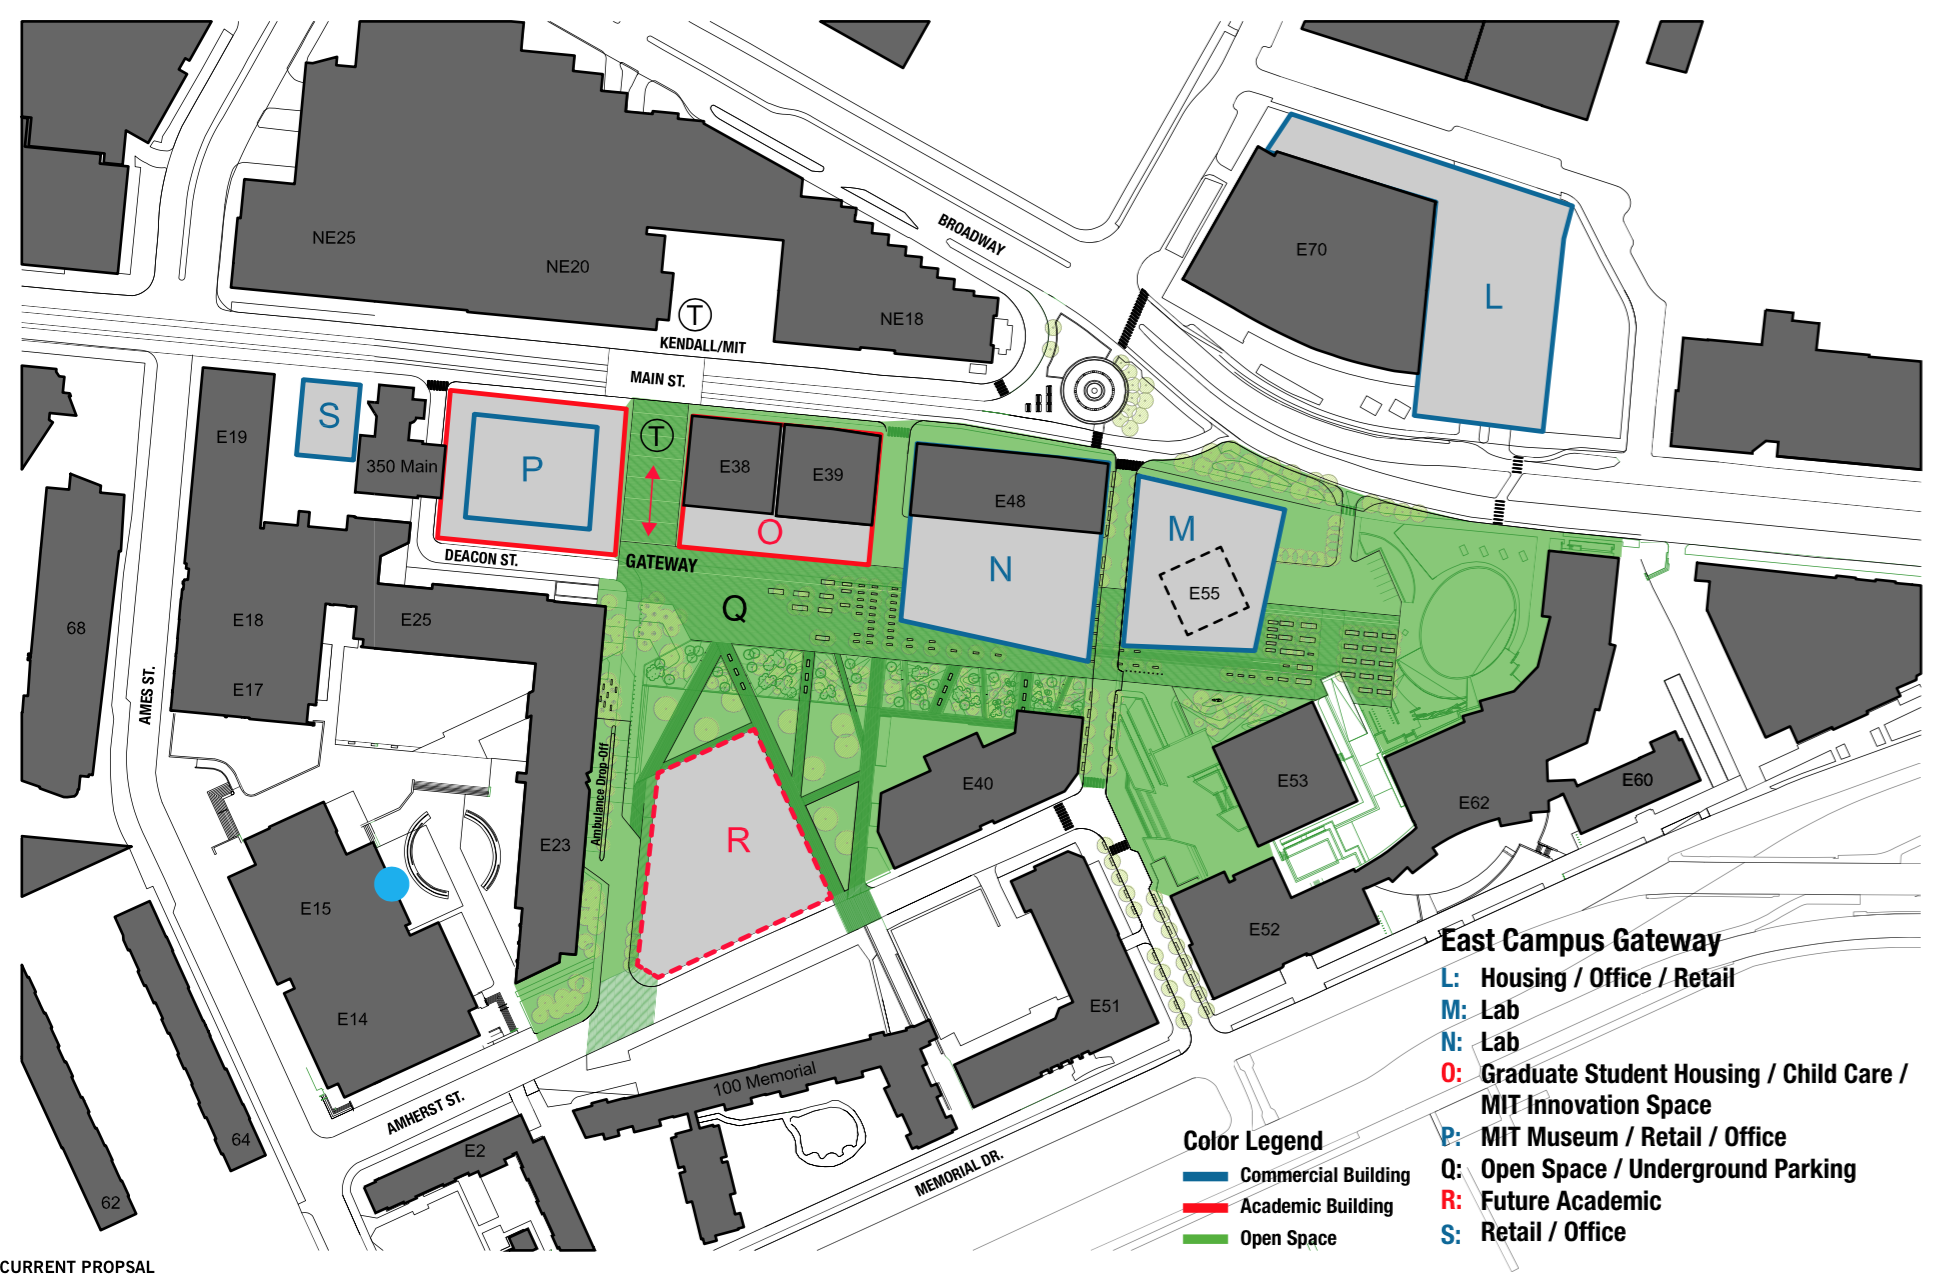
\includegraphics[width=.75\textwidth]{chapters/transformation/playground/figures/playground0.png}
            \end{center}
            \caption{Kendall Square and MIT east-campus. CityScope Playground was used in this observational study to investigate the usability of the TRP system in the context of the MIT east-campus redevelopment project (photo: MIT).}
            \label{fig:pg_kendall_site}
        \end{figure}

        \textbf{Site:} Kendall Sq. in Cambridge, MA, was chosen for this case study. The unique features of this area\footnote{Kendall Sq. is sitting on the verge of MIT, has adjacency to low-density, low-income neighborhoods, close to Boston CBD, and surrounded by unique geographical features.} creates additional interest for the study of regulatory frameworks and their impact on new development (see Figure \eqref{fig:pg_kendall_site} for the redevelopment site used in this study). During the past few decades, the post-industrial area of Kendall Sq. reemerged as a technological hub. Several planning effort were initiated to increase capacity for MIT eastern campus and the adjacent area, aiming to update current height limits, AOR, GFA and other regulations\footnote{See Appendix \eqref{appendix:playground} for the history and a list of redevelopment efforts in the Kendall area.}.
        \newline
        \textbf{Zoning and Regulation:} Kendall Square was intensively planned over the years. Due to its history, location, and unique geography, the site intersects multiple zoning areas. From the south-east, the MIT main campus has mostly low-rise buildings and continuous facades, stretching along Main street and Memorial drive; From the north, a mixture of high-rise office towers, medium-rise condominiums, and low post-industrial structures; In the north-west, low-rise and residential buildings. Over the years, these typologies created a massive trail of zoning and regulations, which can be challenging to distill even by professionals\footnote{An example of this ambiguity could be found in the K2C2 study (Kendall and Central squares), commissioned by the city in early 2011 in response to interest in increased development capacity. Although the study guidelines represent thorough research done in order to improve redevelopment efforts, the legal status of these recommendations is unclear: \begin{quotation} ``The Kendall Square Design Guidelines are created... to \textbf{inform} property owners, business owners, developers, and the general public about the desired form and character of development in Kendall Square...However, the guidelines are not intended to impose a strict limitation on the building form and style. Other creative design solutions, or measures, not noted here may also be utilized to achieve the same goals at the discretion of the Planning Board..." \end{quotation}}.
    }

    \subsection{Tangible Regulation Platform}

    {
        This user study compares two different urban-planning methodologies: (i) Classic, `pen-and-paper' decision-making, and (ii) A digital-physical decision support system. The comparison is meant to enhance the differences between an evidence-based urban-planning session, and a traditional one.
        The Tangible Regulation Platform (TRP) is a CityScope variant designed to evaluate urban-design proposals in the context of zoning-laws and regulations. Users input is examined in real-time, to reflect their impact on the built environment, and to offer an early assessment of the buildable zoning envelopes. For example, a community undergoing a redevelopment initiative, could benefit from the TRP to preform zoning simulation, sometimes years before actual development is taking place. Figure \eqref{fig:pg_trp} shows the TRP setup and usage.
        \newline
        The TRP is composed out of three components: (i) A physical 3D urban model, (ii) a computational unit, and (iii) a feedback module. The computational unit is responsible for evaluating the city regulations and guidelines in response to users input. These algorithms compile zoning, code, and regulations into virtual envelopes, mimicking to the way a municipal board would evaluate a development proposal. Figure \eqref{fig:pg_module} describe the zoning simulation module.
    }

    \begin{figure}[!htb]
        \begin{center}
            \includegraphics[width=0.65\textwidth]{chapters/transformation/playground/figures/playground2.png}
        \end{center}
        \caption{The `zoning simulator'. (from the top) A subset of the zoning amendments proposed for this site was used for modelling the TRP. The zoning codes and building regulations were converted to logical methods (center), and then linked to other methods to evaluate each design proposal. Finally, the results of the simulation was visualized (bottom).}
        \label{fig:pg_module}
    \end{figure}

    \subsubsection{The TRP TUI}
    {
        The TRP includes (i) an array of tagged 3D objects, serving as massing elements of zoning envelopes, (ii) a table that constrains the placement of 3D objects into an urban context, (iii) sensors for scanning the scene, computers, display screens, and projectors for projecting light patterns onto the table. The TRP tabletop is composed of a physical grid of 192x192 LEGO bricks; The grid represents two conditions: (i) `fixed': the non-modifiable parts of the city, and (ii) the `playground': the interactive part of the TRP. A user places physical objects into indentations which form a grid on the table; The objects are then scanned and digitally reconstructed (see Section \eqref{subsec:csarch-cityscopy} for technical description of scanning and parsing the table's state).
        \newline
        Similar to digital monitors, the `resolution' of the table - the density of pixels for a given area - is a key parameter which dictates interaction, simulation, and feedback. Unlike meticulously crafted urban maquettes, the `roughness' of the pixelated CityScope model is intentionally shifting the focus from design details to the overall scheme, massing, and relationships between functions.
        When designing the platform, the smallest tile should represent the smallest unit of interaction and analysis. This decision stems not only from the physical aspects of the urban context, but also from the smallest analytical unit. In the case of the TRP platform, this measurement was based on the smallest unit being used in the site's zoning documents, equal to ~8ft\footnote{The smallest unit was found in an 8ft setback rule, imposed on low-rise building parcels of side streets. This rule was set as the smallest sampling unit for the entire urban model and consequently - for the buildings' height and appearance.}.
    }

    \subsubsection{Types System}\label{subsec:playground_types_system}

    {
        A set of rectangular blocks was defined as the `Bank'. The blocks, different in height but equal in their footprint, are a collection of 16 unique `zoning elements'. Each element retains two parameters: land-use and height, and each block can hold more than one land-use; For example, one block with 22 floors may include 3 floors of retail space in the street level, and 19 floors of residential or office space above. Here, a single block cannot represent a building; In order to construct a viable building envelope, each of the given blocks must be attached to others. The assemblage of these blocks creates zoning envelopes that are diverse in size and program, thus creating a complex zoning environment\footnote{CityScope Playground used an early data scheme to represent the table's state and interaction. For the CityScope Schema, see Section \eqref{sec:cityscope_architecture}.}.
    }

    \subsubsection{Feedback Module}

    {
        \textbf{Scanning And Evaluation:} When users change the configuration of the 3D objects array, the digital reconstruction of the CityScope grid is analysed in relations to the zoning and regulation. The output of this analysis is plotted as a visualization to both the tabletop and a set of vertical monitors. The users then react to the feedback in their next interaction with the TRP.
        \newline
        \textbf{Feedback Devices:} The TUI setup consists of two output devices: Array of 4 projectors, mounted to the room's ceiling above the table corners; The projectors are synced to the 3D models shape using projection mapping. The projectors display data visualization corresponding to users` interaction, so that changes made to the physical model will be visually echoed.
        The second part of the feedback module is a TV dashboard, synced with the projected visualization. Information displayed on the screen is (i) GFA calculation for new additions and for existing urban context; (ii) Percentage of buildings using or exceeding existing FAR; (iii) Open space and built-area ratios; (iv) Occupancy and sub-sectioning of each land-use.

    }

    \subsection{Observational Study}

    {
        The observational study was conducted with a representative sample of users from different backgrounds. The users were randomly invited to examine the usability of the TRP, and to express their opinion on ways to improve planning processes through such platforms. The sessions involved decision-making and design scenarios using artifacts such as paper-based sketching, note-taking, as well as verbal discussions. All sessions were recorded and analyzed; A coding scheme was developed for analyzing the video observations, in order to examine the wide spectrum of actions, verbal cues, and non-verbal gestures, as well as quantify the occurrences of these interactions during the experiment.


        \begin{figure}[!htb]
            \begin{center}
                \includegraphics[width=1\textwidth]{chapters/transformation/playground/figures/playground1.png}
            \end{center}
            \caption{CityScope Playground and the TRP. (right) Overview of the complete system, including the TUI, feedback module, and the `Bank'. (left) The TUI in use during the experiment. Users can collaboratively interact, discuss, and improve their design based on feedback from their peers and the system's responses.}
            \label{fig:pg_trp}
        \end{figure}

        Fifteen participants from the MIT community, including students, staff, and affiliates were invited through an open, unrestricted online form, email lists, and in-campus publications. Upon arrival, the participants were divided into two groups: \textbf{Community Meeting session:} This group held a paper-based discussion, and later moved to the \textbf{TRP session:} In which participants were invited to use the interactive tangible model.  Recording was done using Morae \cite{techsmit94:online}, a usability testing tool to record and analyze multiparty sessions.


        \subsubsection{Procedure}
        {
            In each of the sessions, participants were asked to respond to real-life planning and design challenges in the Kendall Sq. area. At the beginning of the day, the groups were informed about past and existing master-plans and zoning restrictions imposed on the site. They were then asked to rebuild and plan the Kendall Sq. area, taking into account zoning restrictions by adding residential, commercial buildings, parking lots, parks and public amenities. In the TRP session, participants were asked to do the same, while interacting with the CityScope platform. The TRP real-time feedback notified the user whenever a violation of the zoning restrictions occurs in their design, through visualization, text, and symbols.
        }




        \begin{figure}[!htb]
            \begin{center}
                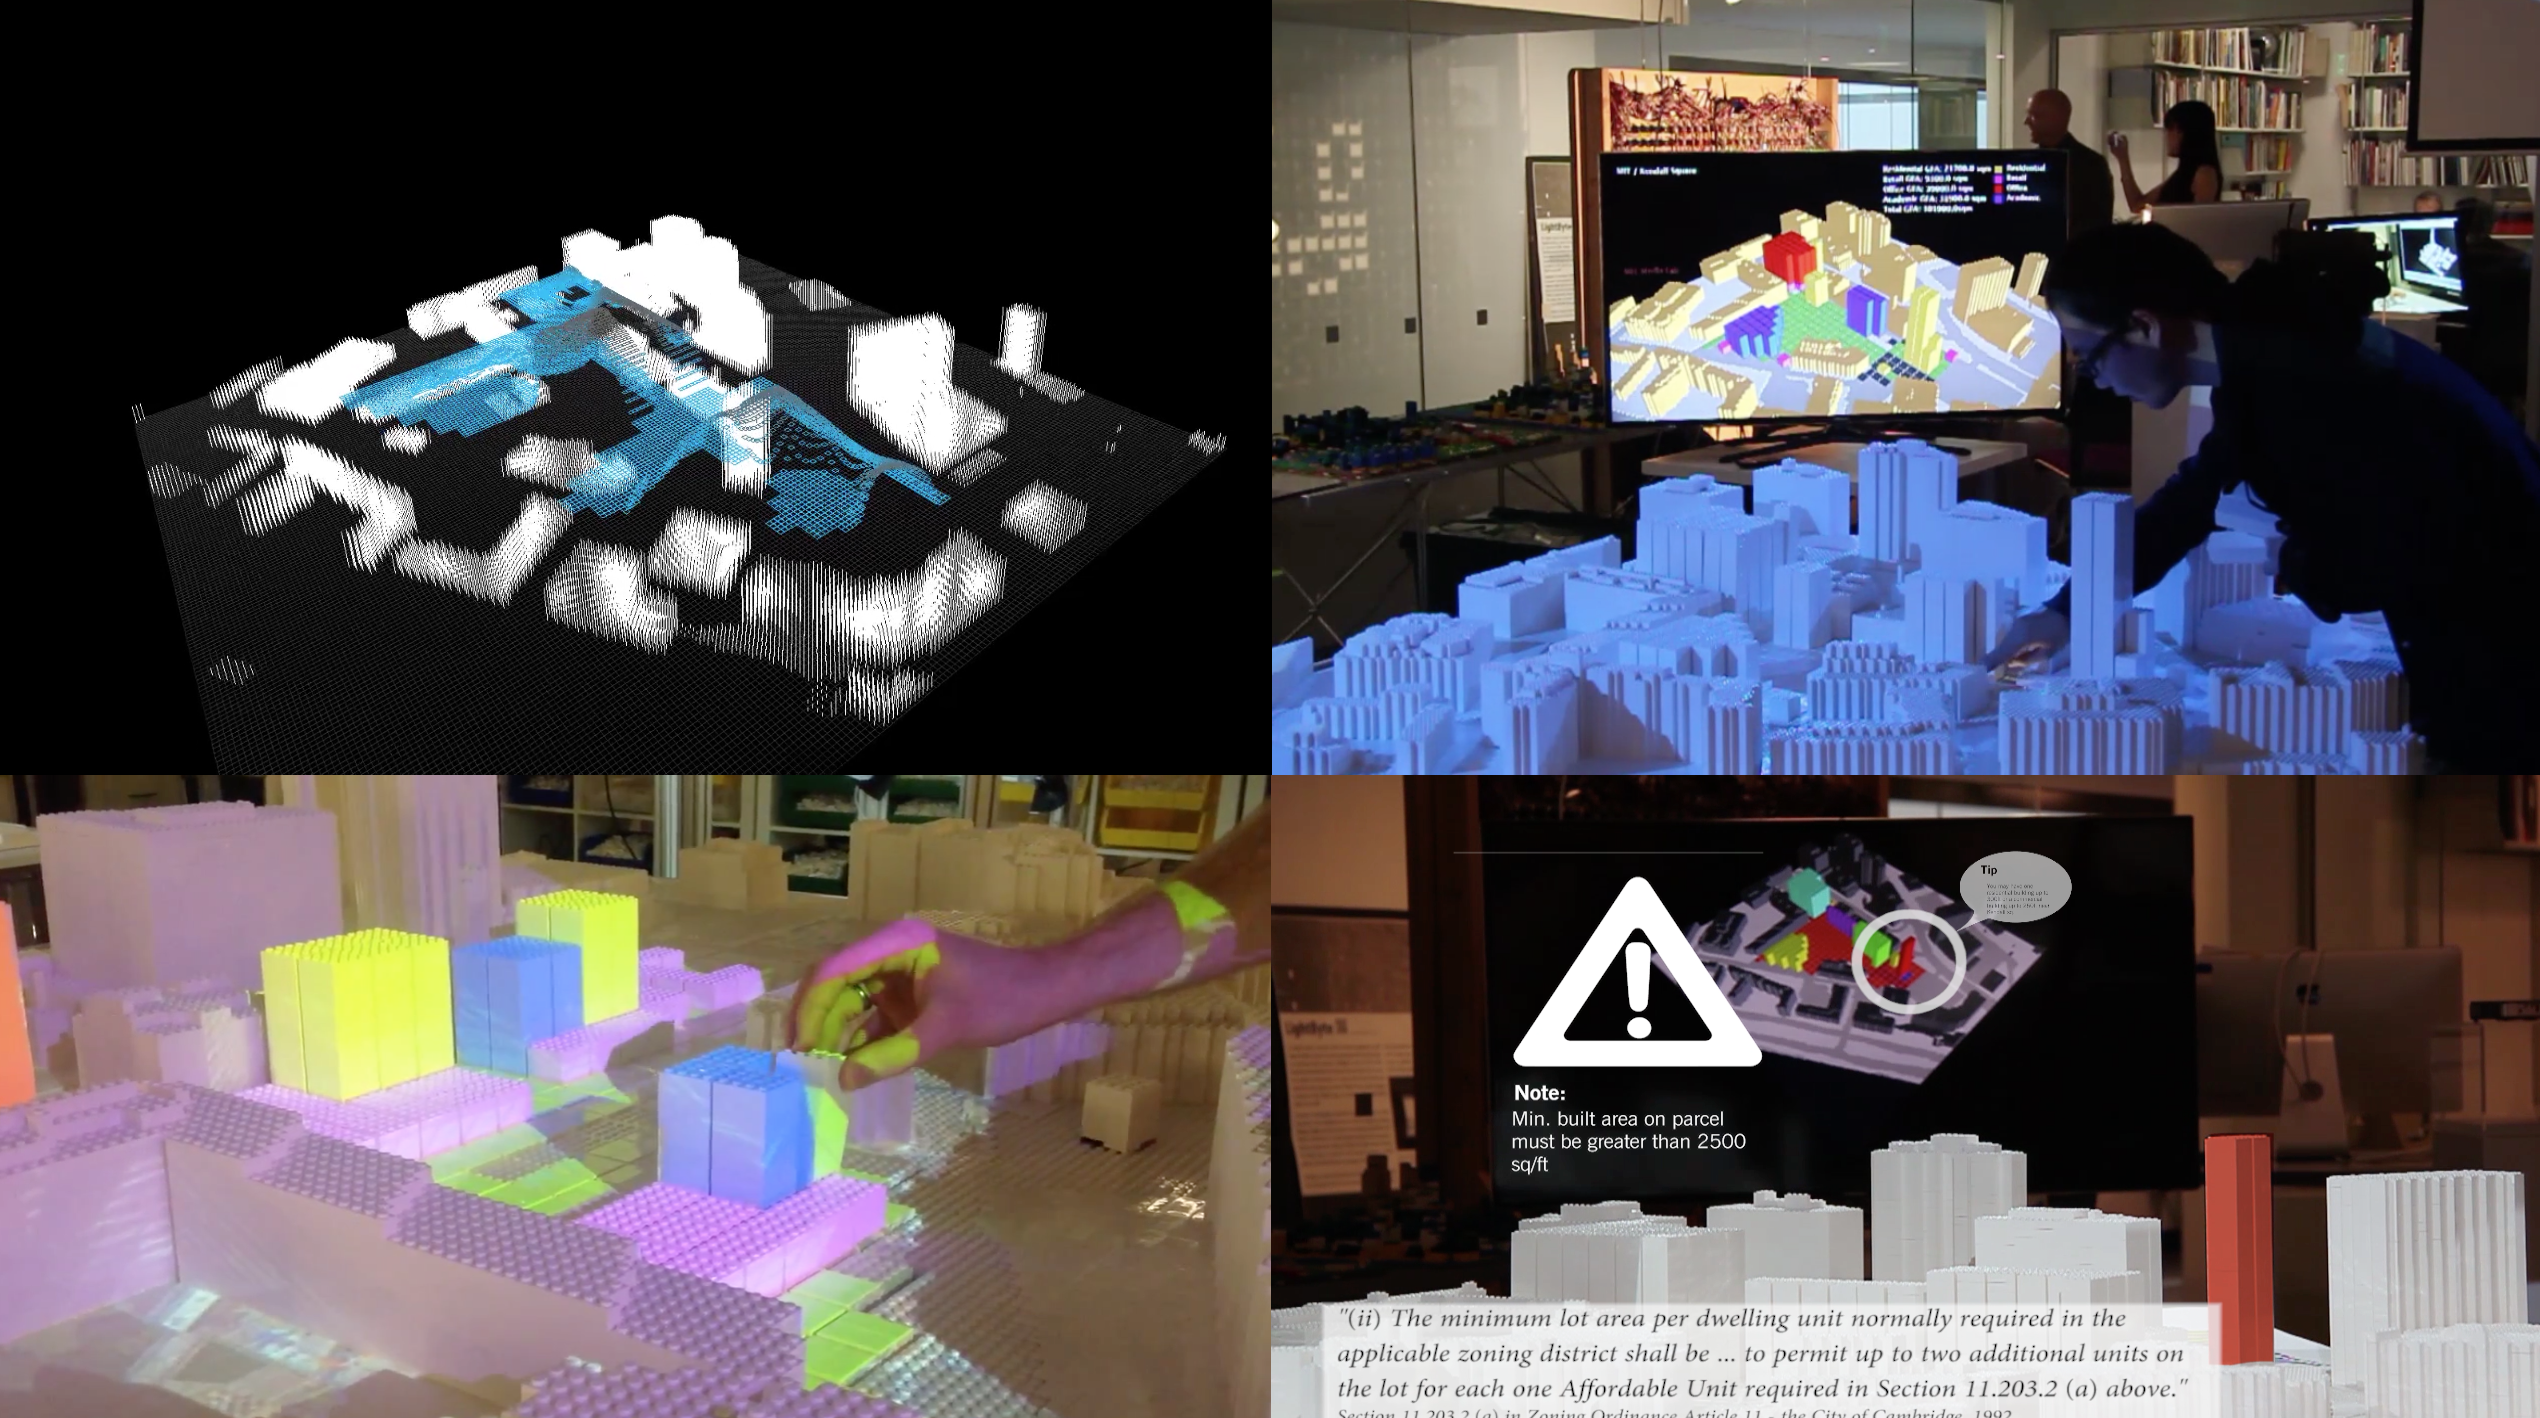
\includegraphics[width=1\textwidth]{chapters/transformation/playground/figures/playground3.png}
            \end{center}
            \caption{User interaction and TRP feedback. As users interact with the TRP, the system evaluates the design based on the zoning simulator module. As users progress with their spatial design, the system highlights violations of the zoning-laws and building-codes, allowing the user to align their design or otherwise challenge the zoning rules.}
            \label{fig:pg_interaction}
        \end{figure}


        \subsubsection{Analysis}

        {
            The video recordings of the sessions were analyzed using a coding scheme. The different types of coding schemes, actions, verbal and non-verbal behaviors are described in Table \eqref{tab:coding_scheme}; Results of the analysis are presented in the Appendix Table \eqref{appendix:coding_scheme_results}.

            \begin{table}
                \begin{center}
                    \caption{Coding Schemes}
                    \label{tab:coding_scheme}
                    \begin{tabular}{l|ll|ll}
                        Code & Description           & Code & Description                              & \\

                        \noalign{\hrule height 0.5pt}

                        EXP  & Explore Function/Tool & EXT  & Excitement                               & \\
                        PUZ  & Puzzled               & SUR  & Surprised                                & \\
                        CLA  & Clarification of Idea & ACT  & Wrong Action                             & \\
                        IDE  & Introduction of Idea  & FRT  & Frustration                              & \\
                        ACC  & Acceptance of Idea    & DIS  & Discontinuous Action                     & \\
                        EVA  & Evaluation of Idea    & REC  & Recognition of Error or Misunderstanding & \\
                        REF  & Refinement of Idea    & DBT  & Doubt                                    & \\
                        HAN  & Hand over             & COR  & Corrective Action                        & \\
                        HES  & Hesitation            & FLO  & Floor-Holding                            & \\
                        DIF  & Execution Difficulty  & TAS  & Give Task to Another User                & \\
                        EXE  & Execution Problem     & SCH  & Search for Non-Existing Function         &
                    \end{tabular}
                \end{center}
            \end{table}
        }
    }

    \subsection{Results and Findings}

    {
        The video recordings of each session was analyzed using the predetermined coding scheme. This scheme included several types of actions, verbal and non-verbal behaviors, and physical gestures. The coding scheme helped recognizing behavioral patterns in the different sessions. For example, it was apparent that most participants spend the first part of their session exploring the TRP and searching its basic functionality, as noted by the multiple occurrences of $EXP$ and $SCH$ codes. Therefore, it can be assumed that a demonstration of the system would make users more comfortable interacting with it. The occurrences of code $IDE$ indicates that dealing with physical objects made participants more active and engaged in the planning and decision-making process. The $ACC$ code reflects that due to the feedback visualization, participants shared a common understanding of the proposed plan. As indicated in the multiple occurrences of $CLA$ and $EVA$ codes, the attention to zoning violation was greater while using the TRP due to real-time feedback. Unlike traditional sketching methods, where participants might not consider zoning, the TUI assisted participants in identifying violations of the zoning restrictions.
        \newline
        In terms of TUI design, the systems was found to cause some frustration and confusion (which is noted in codes $FRT$ and $PUZ$) when participants could not differentiate between removable and fixed physical objects, and when they indicated difficulties in identifying an object. These observations revealed opportunities for improving the user experience of the TUI system\footnote{For full breakdown of the coding scheme results, see Table \eqref{tab:coding_scheme} in the Appendix.}.
    }


    \subsection{Discussion}
    {
        In order to design successful UHCI systems that supports collaboration and facilitate decision-making between stakeholders, it is essential to test their usability in real-world scenarios.
        This study analyzes the usability of a Tangible Regulation Platform (TRP) system, by applying a coding scheme on recorded observations of users' experience, and decoding them to asses usability, and interaction. These findings suggest that UHCI are superior to traditional urban-planning methods in terms of rapid prototyping, collaboration, and decision-making processes.

        \subsubsection{Strengths}
        {
            The TRP platform had several key technological and operational advancements over prior art: This platform was the first large scale CityScope that incorporated real-time interaction, feedback, and participation, all in one system. Despite analyzing unconventional metric such as zoning laws, the TRP feedback was proven to be effective in user experiments.
        }

        \subsubsection{Challenges}

        {
            Evaluating the platform within the confines of the Media Lab building had several limitations. First, intervention in an existing urban-design proposal should involve stakeholders or communities that have direct relations to the site in question. Amongst the visitors, only few were local residents who generally shared a wide and inconsistent degree of acquaintance with the site.
            Second, the TRP zoning analysis could not be evaluated against the actual process of zoning evaluation by the city. In later CityScope projects, evaluations and analysis would be comparative to the actual evaluation process (for example, see the Grasbrook project \eqref{sec:grasbrook}).
        }

        \subsubsection{Opportunities}
        {
            A key finding emerging from both formal and informal feedback, was that participants desired to not only use the TRP to evaluate zoning, regulations, and building-code, but also to use it for other urban performance metrics. As such, municipalities or public officials may test walkability and transportation concerns; The quality of open landscapes, public amenities and civic safety can be tested in existing or amended regulations; Potential ROI, revenues, or market-appeal of properties can be assessed prior to regulatory amendments.
        }
        \newline
        These findings paved the way to a more holistic approach in the design, development, and deployment of future CityScope platforms. The rest of this Chapter details a unified CityScope platform which is set to answer multiple spatial questions, and to be used by multiple stakeholders, settings, and stages of the planning process (see \eqref{sec:cityscope_architecture}, \eqref{sec:grasbrook}).

    }
}
    %%%%%%%%%%%%%%%%%%%%%%%%%%%%%%%%%%%%%%%%%%%%%%%%%%
    \section{CityScope Volpe}\label{sec:cityscope_volpe}
{
    \subsection{Introduction}

    {
        Building upon the PlayGround-TRP project \eqref{sec:cityscope_playground}, this work extends CityScope with different layers of information and real-time analytics. The urban context for this project was the Volpe site in Cambridge, MA, which in 2016, was still vacant and set for redevelopment. CityScope Volpe was designed to explore the impact of different interventions, both within the site and its surrounding context, with three primary objectives: (i) To communicate complex urban data and the inter-relationships between urban systems; (ii) To simulate the impact of urban interventions; (iii) To support decision making in an iterative process using a tangible interface. Figure \eqref{fig:volpe_overall} shows CityScope Volpe, the TUI, and the real-time metrics.
    }

    \begin{figure}[!htb]
        \begin{center}
            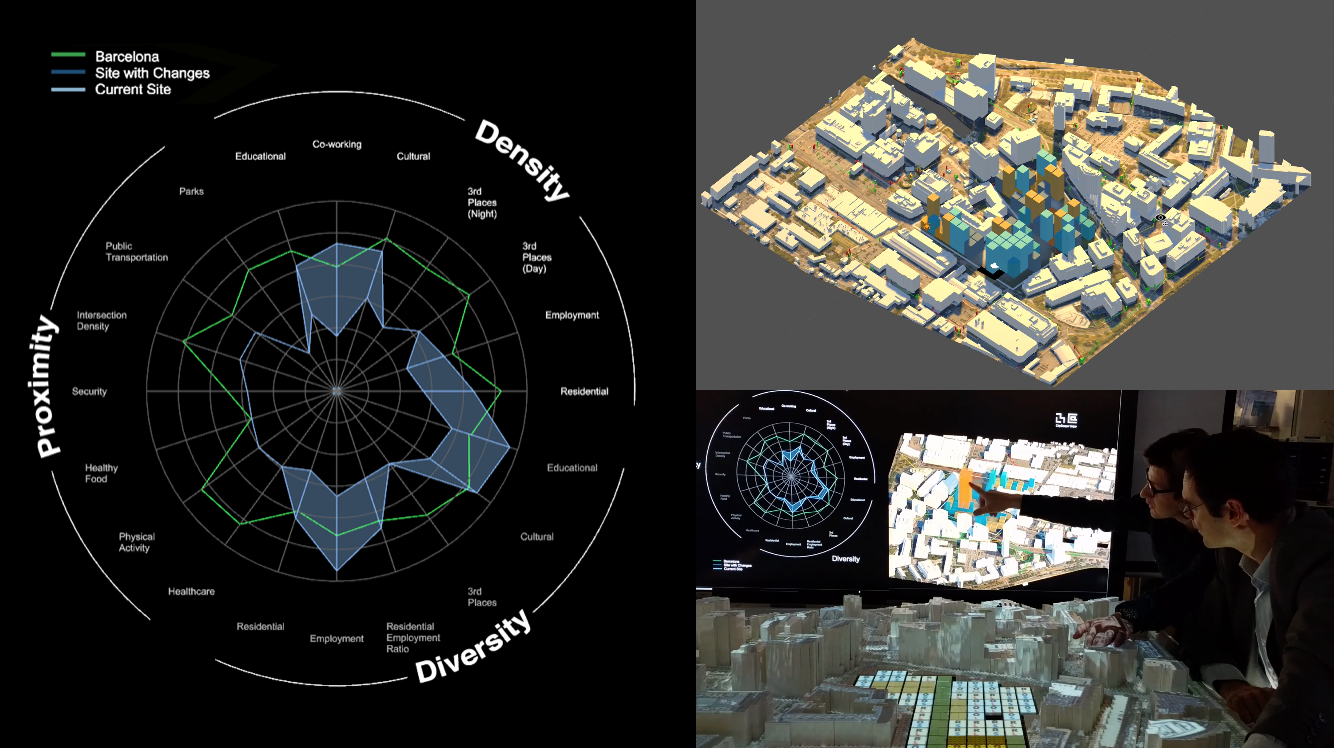
\includegraphics[width=1\linewidth]{chapters/transformation/volpe/figures/volpe0.png}
        \end{center}
        \caption{CityScope Volpe. (left) a set of KPIs and urban indicators are evaluated with each design iteration. (upper-right) The users interactions are translated to three-dimensional zoning envelops, which represent the maximal intervention framework, rather than actual building volumes. (lower-right) Users are presented with both outputs as a mean to direct their design collaboration process.}
        \label{fig:volpe_overall}
    \end{figure}

    \subsection{Site and context}
    {
        As discussed in the previous project \eqref{appendix:playground}, Kendall Sq. was going through extreme urban transformation, driven by the proximity to MIT, Harvard, and the many industries in this area. A limited housing stock and high land values made most residential opportunities in the area out of reach: With a residential density of $\sim$3,000/km$^2$, most workers commute long distances from the greater Boston area, at the cost of energy and time \cite{blanding_blanding_2016}. Additionally, affordable housing incentives were inadequately promoting the necessary range of housing options, and the zoning ordinance has overly restrictive land-use requirements \cite{noyman2015powerstructures}. Alongside low residential density, is the scarcity of services, amenities and 3rd-places, which tend to indicate the urban vitality of a place \cite{Glaeser2011, banerjee2011companion}.
    }

    \subsection{Method} \label{subsec:vople_cityscope}

    {
        CityScope Volpe was built to investigate the redevelopment of the 14-acre DOT facility site, purchased by MIT in 2019 \cite{mit_news}. The physical 3D model is built using LEGO and covers a region of $1km^2$ at a scale of 1:762m\footnote{each 4x4 LEGO tile represents a 26.7 x 26.7 meter area, or 6.675m per LEGO stud.}. Similar to the TRP \eqref{sec:cityscope_playground}, the interactive portion of the model is integrated into the surroundings to represent the area under development, as shown in Figure \eqref{fig:volpe_site}. This intervention region utilizes `CityMatrix' \cite{zhang2017citymatrix}, a Rhino-Grasshopper script \cite{TheHisto40:online} for scanning and virtually reconstructing the interactive site. Interchangeable LEGO tiles represent different land-uses ranging from roads, parks, amenities, residential or office buildings. The TUI also includes physical components with sliders and toggles to change the building height and switch between alternative mobility modes. These modifications are recorded and passed to the computational analysis unit in order to provide real-time feedback to the user. The next section describes the different metric computed by the platform, and the different auxiliary tools and software used to compute them.
    }


    \begin{figure}[!htb]
        \begin{center}
            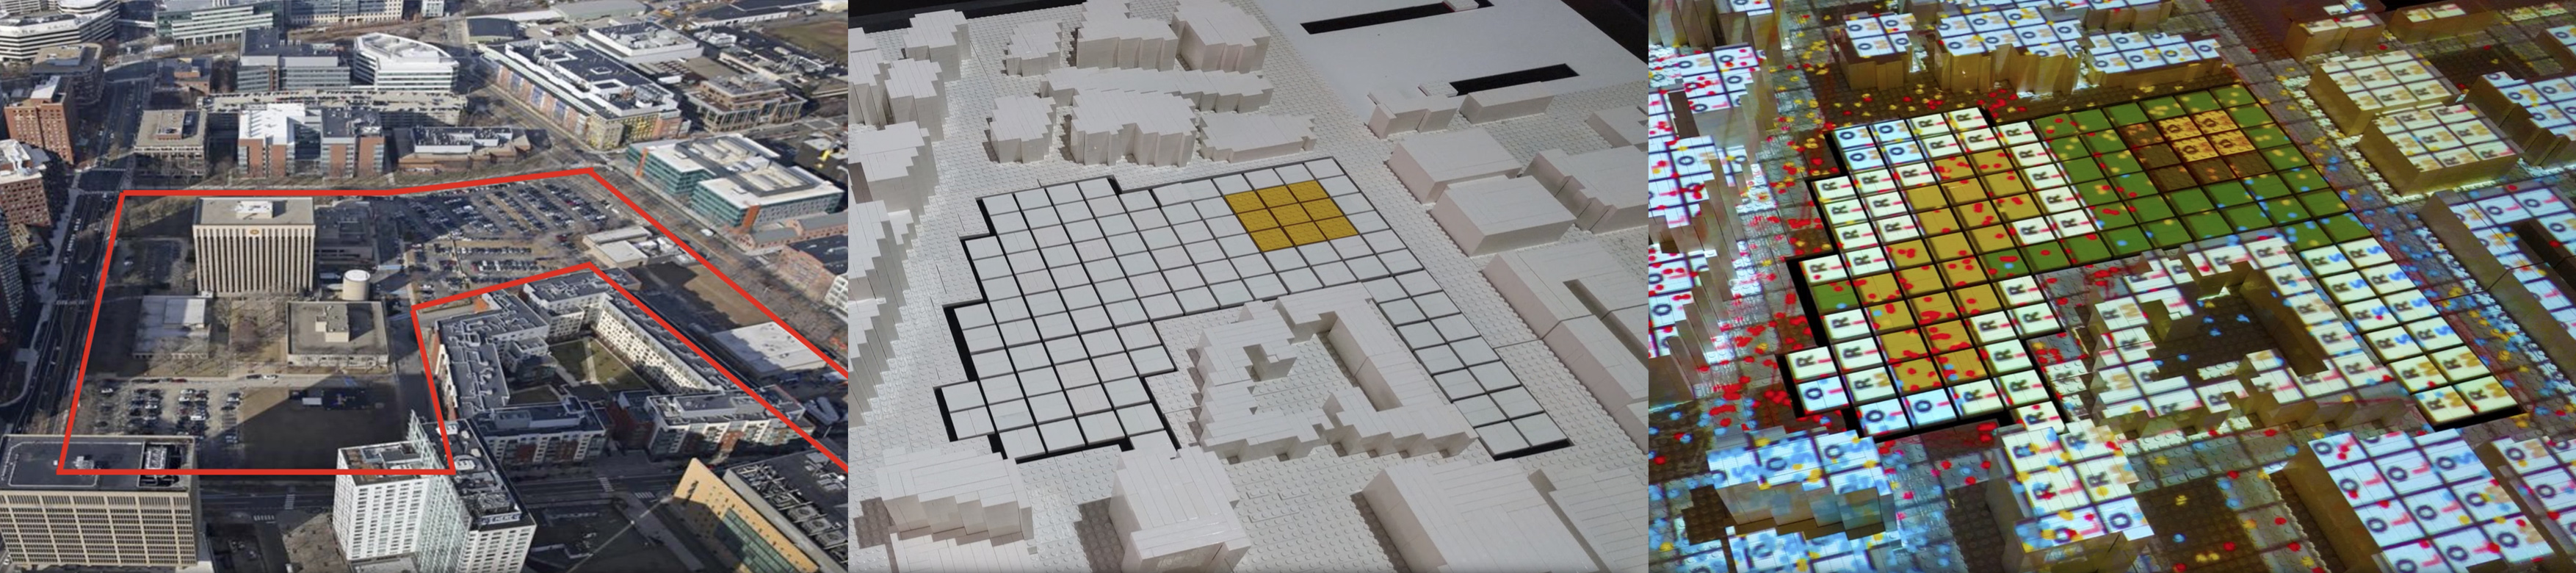
\includegraphics[width=1\linewidth]{chapters/transformation/volpe/figures/volpe3.jpg}
        \end{center}
        \caption{The DOT Volpe facility site. The redevelopment site is abstracted to the CityScope grid, in which the context is immutable and the site is interactive.}
        \label{fig:volpe_site}
    \end{figure}

    \subsection{Urban Performance Indicators}

    {
        In CityScope Volpe, urban performance is analyzed in terms of social, economic and physical attributes, which are clustered as Density, Diversity, Proximity, Mobility, Building Energy and Innovation Potential \cite{katz2014rise}. The computational analysis uses a number of tools to calculate a range of performance metrics, and produces feedback in the form of both spatial and numerical statistics, including Rhino-Grasshopper, GAMA platform, and Unity \cite{TheHisto40:online, grignard2013gama, UnityRea35:online, noyman2018CityScopeARUD}. The different urban performance indicators are shown in Figure \eqref{fig:volpe_overall}. The rest of this section overviews the different metrics and indicators used in the analysis.

        \subsubsection{Density}
        {
            The ratio between housing, commercial space, retail venues, cultural institutions, and other amenities is known to be related to the creation of well functioning cities \cite{lynch1984good, gehl2013study, katz2014rise}. Density has to be balanced in order to ensure positive outcomes (such as greater exchange of ideas, economic mobility, more employment options, better amenities, or energy reduction) with fewer negative outcomes (such as traffic congestion, lack of natural resources, or pollution) \cite{hawley1972population, UnitedNationsHabitatIII2017, deloitte_2021}. In Volpe, the density of each land-use type (eg. amenities, residences, employment) can be represented as $Density^m=\frac{|M|}{A}$, where $M$ is the set of occurrences of $m$ in the design area, and $A$ is the total area of district.
        }


        \begin{figure}[!htb]
            \begin{center}
                \includegraphics[width=1\linewidth]{chapters/transformation/volpe/figures/volpe2.png}
            \end{center}
            \caption{User interaction and feedback. As users interact with the CityScope TUI, urban performance indicators update in real-time: density, diversity, proximity, mobility energy per person, walkability, access to parks, and a simulated probability of meeting areas (so called `collision potential').}
            \label{fig:volpe_layers}
        \end{figure}

        \subsubsection{Diversity}
        {
            Highly performative urban areas tend to present an increased diversity of social, economic and spatial characteristics. The Diversity index is assessed using a Shannon-Weaver formula \cite{kemeny2013immigrant} and Balanced Ecosystem index: Quantitative measurement that reflects how many different types (species) there are in a certain set (community/ecosystem), and simultaneously takes into account how evenly the basic entities (individuals) are distributed among those types. This can be represented as $H = - \displaystyle\sum_{i=1}^{S} p_i ln p_i$, where $H$ is the Shannon diversity index, $S$ is the total number of species in the community, and $p_i$ is the proportion of the population made up of species $i$. Naturally, not all species are - or should be - equally represented, and the diversity index only measures the distribution of these species.
        }

        \subsubsection{Proximity}

        {
            Proximity assesses the accessibility and closeness indexes between social, economic and physical functions in urban environments \cite{sevtsuk2016pedestrian}. Historically, high performing cities resemble networks of compact urban districts where resources and amenities of daily life are in close proximity to one another \cite{westerink2013dealing}. In Volpe, proximity metrics include walkable access to parks, housing, jobs, mass transit, schools, and amenities. For a given `goal object', a proximity metric for a district can be calculated as $Closeness\,to\,SM = (\sum\limits_{j\epsilon B_i} dist(j,closest(j,SM)))^{-1}$, where $B_i$ is the set of tiles in district $i$, $SM$ is the `goal' objects (Parks, Residential, Office, etc.), $dist (a; b)$ is the geographical distance between two elements' centroids $a$ and $b$, and $closest (j;Y)$ is geographically closest element in set $Y$ from block $j$ centroid. Figure \eqref{fig:volpe_layers}(top) shows the proximity metric for parks in the Volpe site as a heatmap over TUI.
        }

        \subsubsection{Mobility Energy}
        {
            Several mobility metrics are introduced in this project. An Agent Based Model (ABM) simulates a synthetic population in response to changes in land-use and mobility modes, and calculates the energy produces by each trip \cite{grignard2017agent}. The impacts of urban mobility on energy consumption can be calculated as $E_m = \sum_{m \in M}\sum_{l \in L}v_l^m s_{l} e^m$ where $E_m$ is the total mobility energy, $M, L$ is the set of all transport modes and road network links respectively, $v_l^m$ is the number of vehicles of mode $m$ that travel on link $l$, $s_l$ is the length of link $l$, and $e_m$ is the energy usage per unit distance traveled by mode $m$.
        }

        \subsubsection{Building Energy}
        {
            Energy Consumption is calculated for structures in and around the Volpe area using building envelope performance data, orientation, estimated embodied energy, and land-use information. The metric aims to predict how overall energy consumption of the buildings will change given different urban configurations. The model uses a combination of building use, height, and proximity to adjacent structures in order to account for solar gain. The energy efficiency index is found by dividing the total energy metrics of the buildings with the total energy input, \cite{patterson1996energy} \cite{ferrao2013sustainable} so that $Energy\,Efficiency = \frac{\displaystyle\sum(Useful\,\,Energy\,\,Output)}{\displaystyle\sum(Energy\,\,Input)} \times 100\%$, where $Useful \,Energy \,Output$ is the energy output of the buildings and $Energy \,Input$ is the total energy input of the buildings.
        }

        \subsubsection{Collision Potential}
        {
            Collision Potential is an abstract metric to asses the potential degree of interaction between individuals in a given area, as a proxy of land use and mobility patterns. A simulation model creates a spatial graph where individuals roaming the site are nodes, and edges represent interaction over time. This graph is used to asses metrics such as temporal density, diversity, and network centrality. The collision potential between agents of different demographic groups can be defined as $ C_{A,B} \propto \sum_{a \in A}\sum_{b \in B}\delta_{a,b} \quad \forall A, B \in D$, considering $\delta_{a,b} =
                \begin{cases}
                    1, & \text{if}\ s_{ab}^t < s_{max} \text{ for given timeframe }t \\
                    0, & \text{otherwise}
                \end{cases}$
            \newline
            where $C_{A,B}$ is the collision potential between demographic groups $A$ and $B$, $D$ is the set of all demographic groups under study, $s_{ab}^t$ is the distance between agent $a$ and agent $b$ at time $t$, and $s_{max}$ is the maximum separation distance for interaction potential.
        }
    }

    \subsection{Discussion}\label{volpe_discussion}
    {

        CityScope Volpe has been central to the development and deployment of future CityScope platforms. The underlying scanning and analysis system used in the Volpe case-study \cite{zhang2017citymatrix} was later reused in series of workshops and deployments in cities around the world, including Shanghai, Hamburg, and Andorra \cite{noyman2017finding}. The system has been adjusted on an ongoing basis to improve user experience, models, visualizations, and data. The rest of this Section discusses the strength, weaknesses, and potential of this work.

        \subsubsection{Strength}
        {
            The Volpe platform demonstrated the ability to combine multiple layers of urban analytics into one system, and to provide a unified interface for all of available layers. Additionally, Volpe was using an early version of the cityIO server (see Section \eqref{subsec:csarch-cityio}) for message passing between the scanner (Rhino), the ABM (GAMA), and the 3D representation (Unity3D). This was a precursor to the CityScope Schema, and to the holistic approach to the unification of CityScope \eqref{sec:cityscope_architecture}.
        }

        \subsubsection{Challenges}

        {
            Volpe was not designed as a system that could be easily used in a variety of different contexts, nor it could analyze data from a variety of different sources. The system was built as a hybrid of tools and data pipelines, making it challenging to adapt to new data sources, locations, or research questions. Moreover, the design of this system coupled analysis, interaction, and visualization in one asynchronous system, which was noticeable in lags, stability, and overall complexity of development.
            Lastly, the accuracy of some metrics was not validated in a rigorous manner, and was set more as a placeholder for future research. Coupling explicit analysis (such as density, or spatial proximity) with implicit metrics (such as social diversity, or innovation potential) was difficult to validate, normalize, and communicate, and challenged the overall acceptance of such system.
            \newline
            From a technical perspective, using cityIO as an HTTP server for closed-loop system communication was proven inefficient, since messages were sent across the web, only to appear at a nearby client. Moreover, REST API was not a good fit for a real-time TUI system, which is designed to have low latency. As discussed in Section \eqref{sec:cityscope_architecture}, these challenges led to the redevelopment of many of these systems and data structures.
        }

        \subsubsection{Potential}
        {
            Volpe promoted two streams of development for future CityScope projects: (i) The ability to collect, analyze, and display data from multiple sources, in various analytics methods, and with different types of visualization and feedback; (ii) The ability to discuss social, demographic, and environmental factors of the city, alongside classic urban analytics. As the following projects show, these ideas motivated the development of a unified CityScope system, which includes analytics modules for both spatial, temporal, and social questions within a single framework.
        }

    }
}













    %%%%%%%%%%%%%%%%%%%%%%%%%%%%%%%%%%%%%%%%%%%%%%%%%%
    \section{CityScope Grasbrook}\label{sec:grasbrook}

{
    \subsection{Introduction}
    {
        CityScope Grasbrook was commissioned in 2019 by the the City of Hamburg and the HafenCity Company, as part of a unique tender format for a new residential and business district in the Grasbrook, Hamburg, Germany\footnote{CityScope Grasbrook was born out of a cooperation of three institutional partners: (i) HafenCity Hamburg GmbH is a city-owned urban development agency mandated to develop large-scale projects in the city of Hamburg \cite{cgha19, br18}; (ii) the Digital City Science Lab at HafenCity University HCU; and (iii) the MIT CityScope team.}. The Grasbrook project provided a real-world opportunity to develop and test the idea of the unified and open-ended CityScope architecture (see Section \eqref{sec:cityscope_architecture}). CityScope Grasbrook is a digital online tool and participatory process, that provides algorithmic analysis and predictive simulation for early-stage urban-design proposals in a design competition stage. Specifically, the system supports the decision-making of two user groups: (i) City planners, architects, or designers, in the process of developing urban-designs proposals, and (ii) Competition juries when evaluating said proposals. The system provides instant assessment of environmental and spatial impact, such as noise propagation, pedestrian accessibility, or storm-water flooding; When evaluated, CityScope Grasbrook modules were shown to be comparable or better than experts' analysis of the same metrics.



        \begin{figure}[!htb]
            \begin{center}
                \includegraphics[width=1\textwidth]{chapters/transformation/grasbrook/figures/grsbrk5.png}
            \end{center}
            \caption{Competition submissions vs. CityScope interface. Similar to other architectural and design competitions, the Grasbrook's brief specify certain requirements for each design submission. Nevertheless, `creative freedom' and lack of a strict submission format makes it hard to properly evaluate the performance metrics of each proposal. The CityScope interface, on the other hand, is designed for an `apples-to-apples' comparisons, where the user can observe, evaluate, and correct the results of different submissions in one framework.}
            \label{fig:grasbrook_competition_vs_cs}
        \end{figure}

        \subsubsection{Motivation}
        {
            Urban development projects evolve through complex and lengthy processes: From project initiation, via public deliberation and tendering, onto the physical execution of architectural designs. In all of these stages, a multitude of stakeholders, functional requirements, and criteria must to be well coordinated \cite{alexander1990planning}. Within this process, the results of urban-design competitions play a crucial role, as their procedures and outcomes can strongly determine the shape and quality of future urban environments.
            \newline
            In this context, CityScope Grasbrook addresses two use-cases: (i) \textit{During the Design Process:} CityScope is used by design teams in the earliest phases of schematic design (SD), in which crude proposals are drafted to outline functional and spatial features of the area. In this case, the system was designed to rapidly deliver information on the effects of their drafts, to estimate their overall qualitative performance, and to optimize their spatial layout and functional programs. For example, CityScope may instantly provide answers to questions like: \textit{``How does the placement of a certain building influences the propagation of traffic noise in the area?''}
            \newline
            (ii) \textit{During Jury Review:} Here, CityScope is used later in the competition process, when expert juries assess submissions to conclude the winning entry. At this stage, CityScope helps the jurors to evaluate the submissions, to check their compliance with key criteria, and to judge the different proposals on the basis of objective performance indicators. The comparison of design proposals by way of algorithmic analysis benefits an unbiased and transparent assessment process, and can also eases the task of assessing inconsistent or non-standardized submission formats\footnote{Especially in early design phases, these deliverables could vary dramatically, from mix-media and physical models, to perspective drawings and text descriptions \cite{ben-joseph2001}.}.
        }
    }

    \begin{figure}[!htb]
        \begin{center}
            \includegraphics[width=1\textwidth]{chapters/transformation/grasbrook/figures/grsbrk1.png}
        \end{center}
        \caption{Grasbrook site (right) showing the active harbor section in the south-west, and the Veddel neighborhood to the east. (left) Previous design studies for Grasbrook, by Hosoya Schaefer Architects, Zurich.}
        \label{fig:grasbrook_site}
    \end{figure}

    \subsection{`Competitive Dialogue'}
    {
        A ``Competitive Dialogue'' is a bidding framework designed for complex urban development projects \cite{hpg15}. For the Grasbrook site, the bidding was announced EU-wide, and twelve teams (six urban-design and six landscape-design offices) were invited\footnote{The HafenCity Hamburg GmbH who published and managed the tender, acted as an intermediary between ministries, citizens, experts and design teams in order to supply data and feedback for the iterative improvement of their design schemes.}. In phase one, the teams worked independently within their professional domains; After the conceptual phase, six offices were submerged into three mixed teams, who were asked to propose an holistic landscape and urban-design solution. After the second phase, one winning team was selected by a high-level jury in April 2020.
    }



    \subsection{Platform Design}

    {
        CityScope Grasbrook utilized the unified CityScope architecture (see Section \eqref{sec:cityscope_architecture}) as a baseline for the development of a custom set of analysis modules and feedback features. This system design was well suited for the Grasbrook use-case, since it could host a myriad of analytic tools, whose interconnection enables an algorithmic analysis of complex cause-and-effect chains created by urban-design interventions.

        \begin{figure}[!htb]
            \begin{center}
                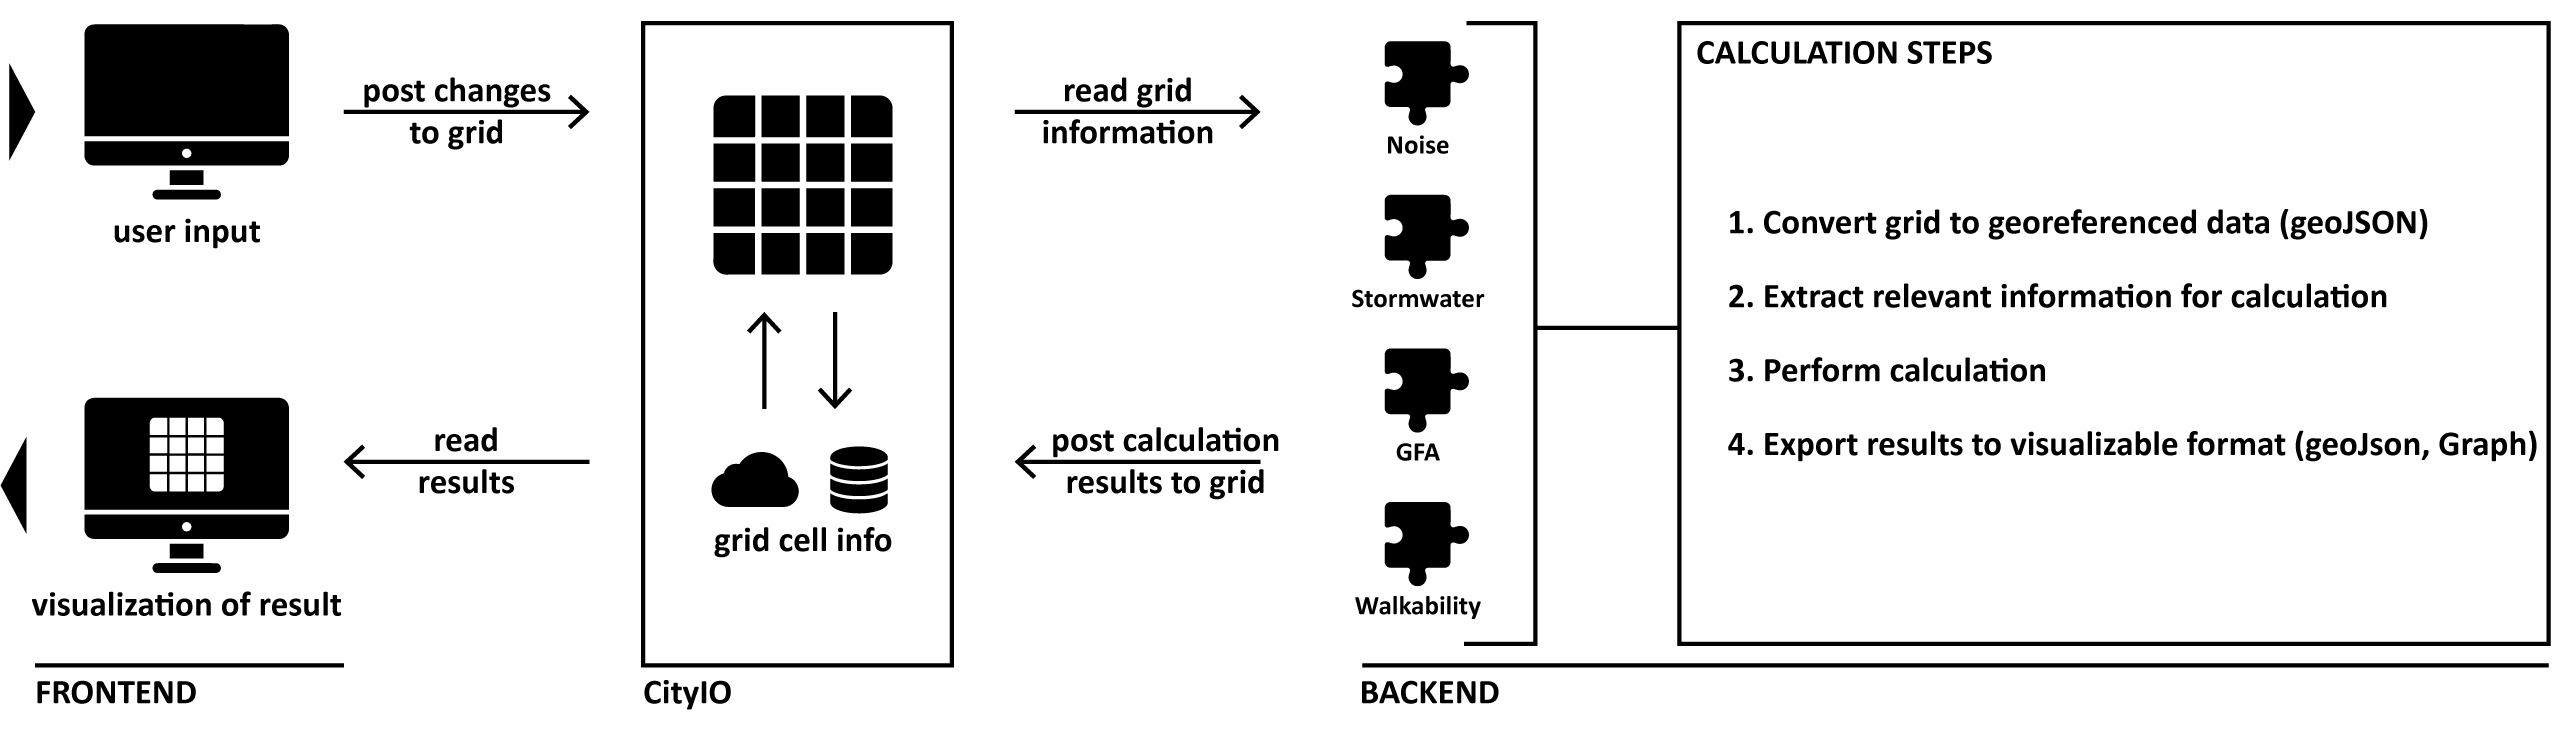
\includegraphics[width=1\textwidth]{chapters/transformation/grasbrook/figures/grsbrk3.jpg}
            \end{center}
            \caption{Grasbrook CityScope System Architecture: Following the CityScope Schema and system design, Grasbrook adapted a parallel data flow between the different components (see Section \eqref{sec:cityscope_architecture}).}
            \label{fig:grasbrook_architecture}
        \end{figure}

        \textbf{Modular Architecture:} CityScope Grasbrook was designed as an online platform first, which could later be extended to TUI and other interfaces as needed. The overall architecture consists of a frontend UI and a set of various backend analysis modules, all of which are connected via cityIO (see \eqref{subsec:csarch-cityio}). With this structure, different software applications for the analysis of specific urban KPIs (i.e. noise propagation, storm-water runoff, pedestrian accessibility) or target indicators (Gross Floor Area, FAR) can be easily plugged-in yet independently developed by different teams.
        \newline
        \textbf{Security Features:} Specific to the Grasbrook case-study, secure storage of the competitors' project data was required. Simultaneous user-access to the CityScope platform, as well as backend data management, had to comply with security and confidentiality standards. Considering legal controversies that sometimes emerge in the aftermath of design competitions, the CityScope team implemented several data security and safety measures: secure user authentications, individual usernames and passwords for each participant, access monitoring, real-time system logging and analytics. These features were implemented in the frontend UI, and the backend cityIO server.


        \begin{figure}[!htb]
            \begin{center}
                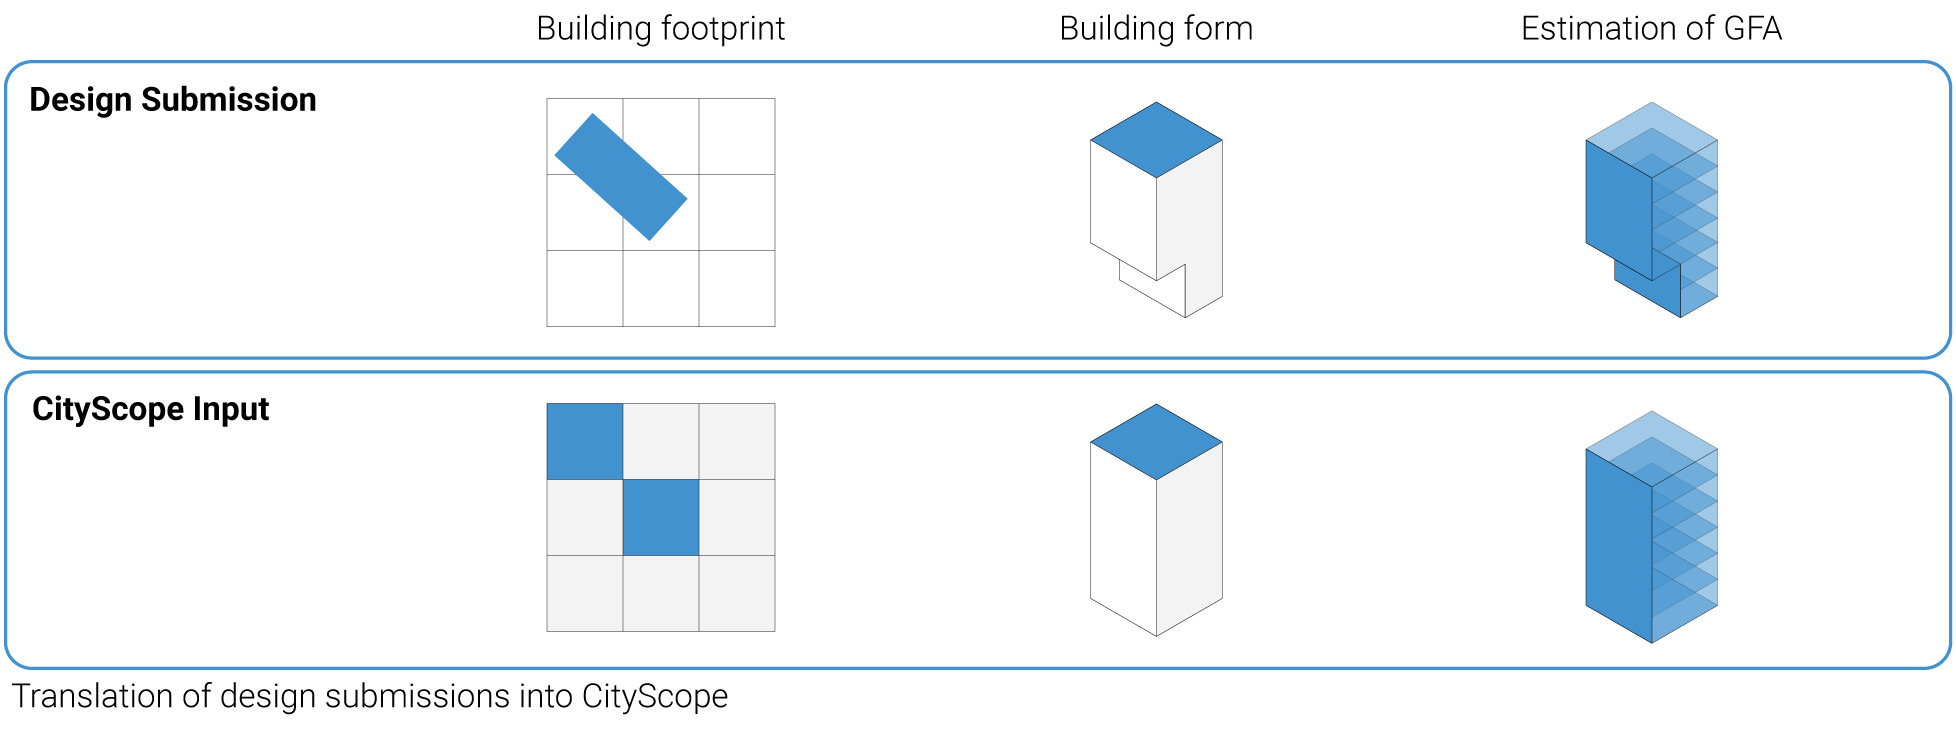
\includegraphics[width=1\textwidth]{chapters/transformation/grasbrook/figures/grsbrk4.jpg}
            \end{center}
            \caption{Translation of design submissions into CityScope grid. When complex shapes are presented, or negative volumes calculation is need for GFA calculations, the grid approach might be less accurate.}
            \label{fig:grasbrook_pixel_translation}
        \end{figure}
    }


    \textbf{Interaction Design:} As with other CityScope projects, site and intervention data is translated into the form of a grid and the CityScope Schema \eqref{sec:cityscope_architecture}, enabling faster modules' calculations and real-time user interaction. This transformation is performed by transferring the morphology of the site into a 2D raster\footnote{in the Grasbrook case, the grid was of 16x16 meters and four meters for ground level, three meters on upper levels}. Each grid cell hold information about its usage (built or unbuilt) along with its core functions (residential, commercial, educational, promenade, street, park, etc.). In the context of the Grasbrook competition, the matrix reflects (i) A standard measure for minimum street width according to heat flow and pollutant dispersion metrics \cite{yc18}; (ii) A building depth allowing natural cross-ventilation and daylight penetration \cite{mn19}; (iii) A suitable level of detail for visualization, allowing intuitive and real-time feedback for user interaction; and (iv) A documented metric for other similar cases of computational urban simulations.


    \subsection{Analytic Modules}

    {
        HafenCity Hamburg GmbH prioritized four types of analytic modules: noise propagation, storm-water runoff, walkability, and gross floor area (GFA). These modules were deemed as key in the decision-making process of the competition, as they commonly hard to infer from the design submission themselves. The following is a description of each module, and an evaluation of its performance and usability.

        \begin{figure}[!htb]
            \begin{center}
                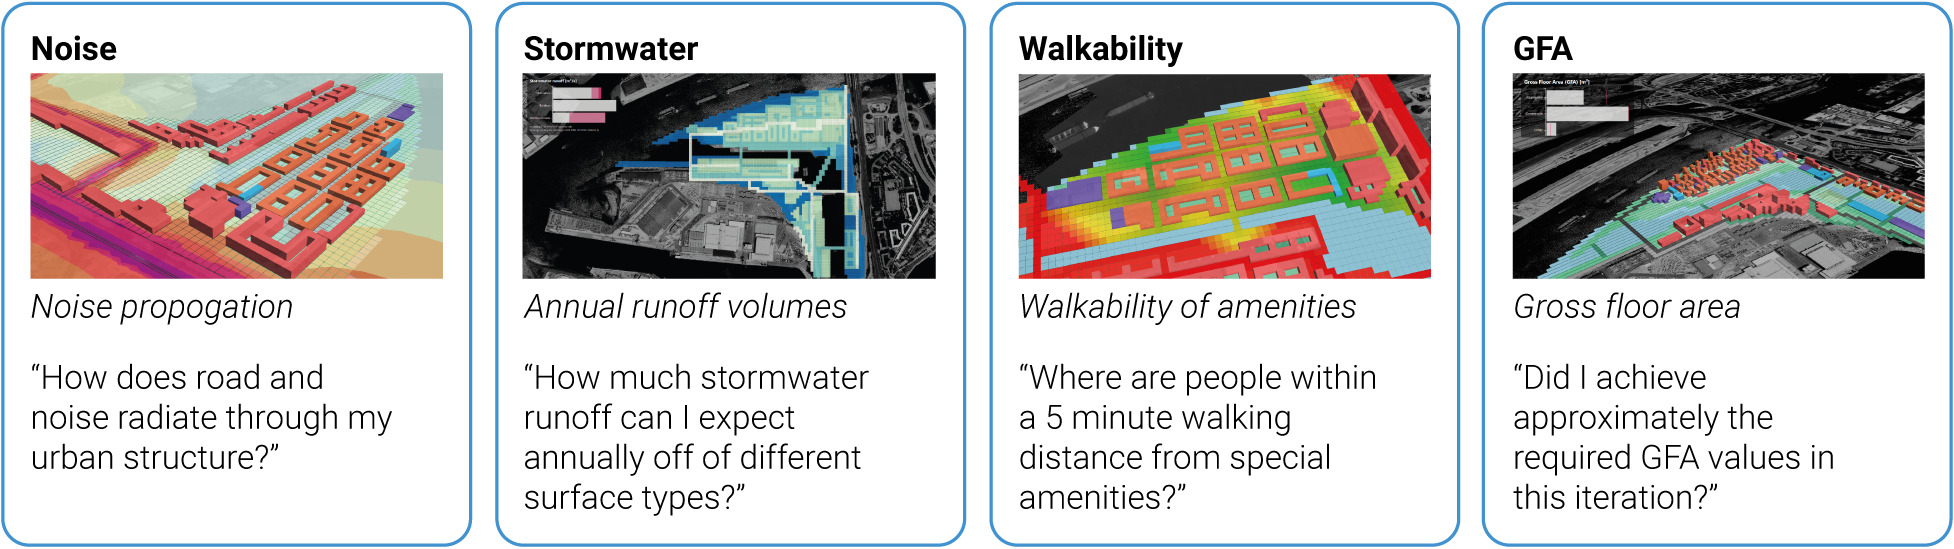
\includegraphics[width=1\textwidth]{chapters/transformation/grasbrook/figures/grsbrk2.jpg}
            \end{center}
            \caption{Goals of each of the CityScope modules used in Grasbrook. As with other CityScope projects, each module should aim to answer a specific question. For CityScope users, the overlapping of different modules' responses creates a deeper understanding of the design tradeoffs, for example: `Would this intervention promote both easier access AND better water management?'}
            \label{fig:grasbrook_modlues_questions}
        \end{figure}


        \subsubsection{Modules Accuracy}
        {
            This project was a first opportunity to test the CityScope modular architecture in real-world use-case. This required a high level assessment of modules' quality and reliability, for both the design teams as well as the jurors. In communications to the design teams, trade-offs between usability, speed of interaction, and quality of assessment were highlighted.
            While higher accuracy and reliability could only come from expert reports and industry standard, these tend to be costly, take substantially longer time to produce, and would not be as iterative as the CityScope layouts. Since CityScope pixelates the raster of the design space, calculating the level of accuracy was done by comparing modules' output with rasterized results of analysis preformed by external committee of experts\footnote{The introduction of CityScope to the Grasbrook tender had to comply with organizational and legal constraints. Due to the academic nature of the project, it was necessary to distinguish the features and outputs of the CityScope solution from those of accredited expert tools. When introduced to the competition teams, the aim and character of the scientific experiment were communicated, and it was maintained that the solution would not deliver legally binding output or assessments, but rather provide additional support for the decision-making process.}.
        }



        \begin{figure}[!h]
            \begin{center}
                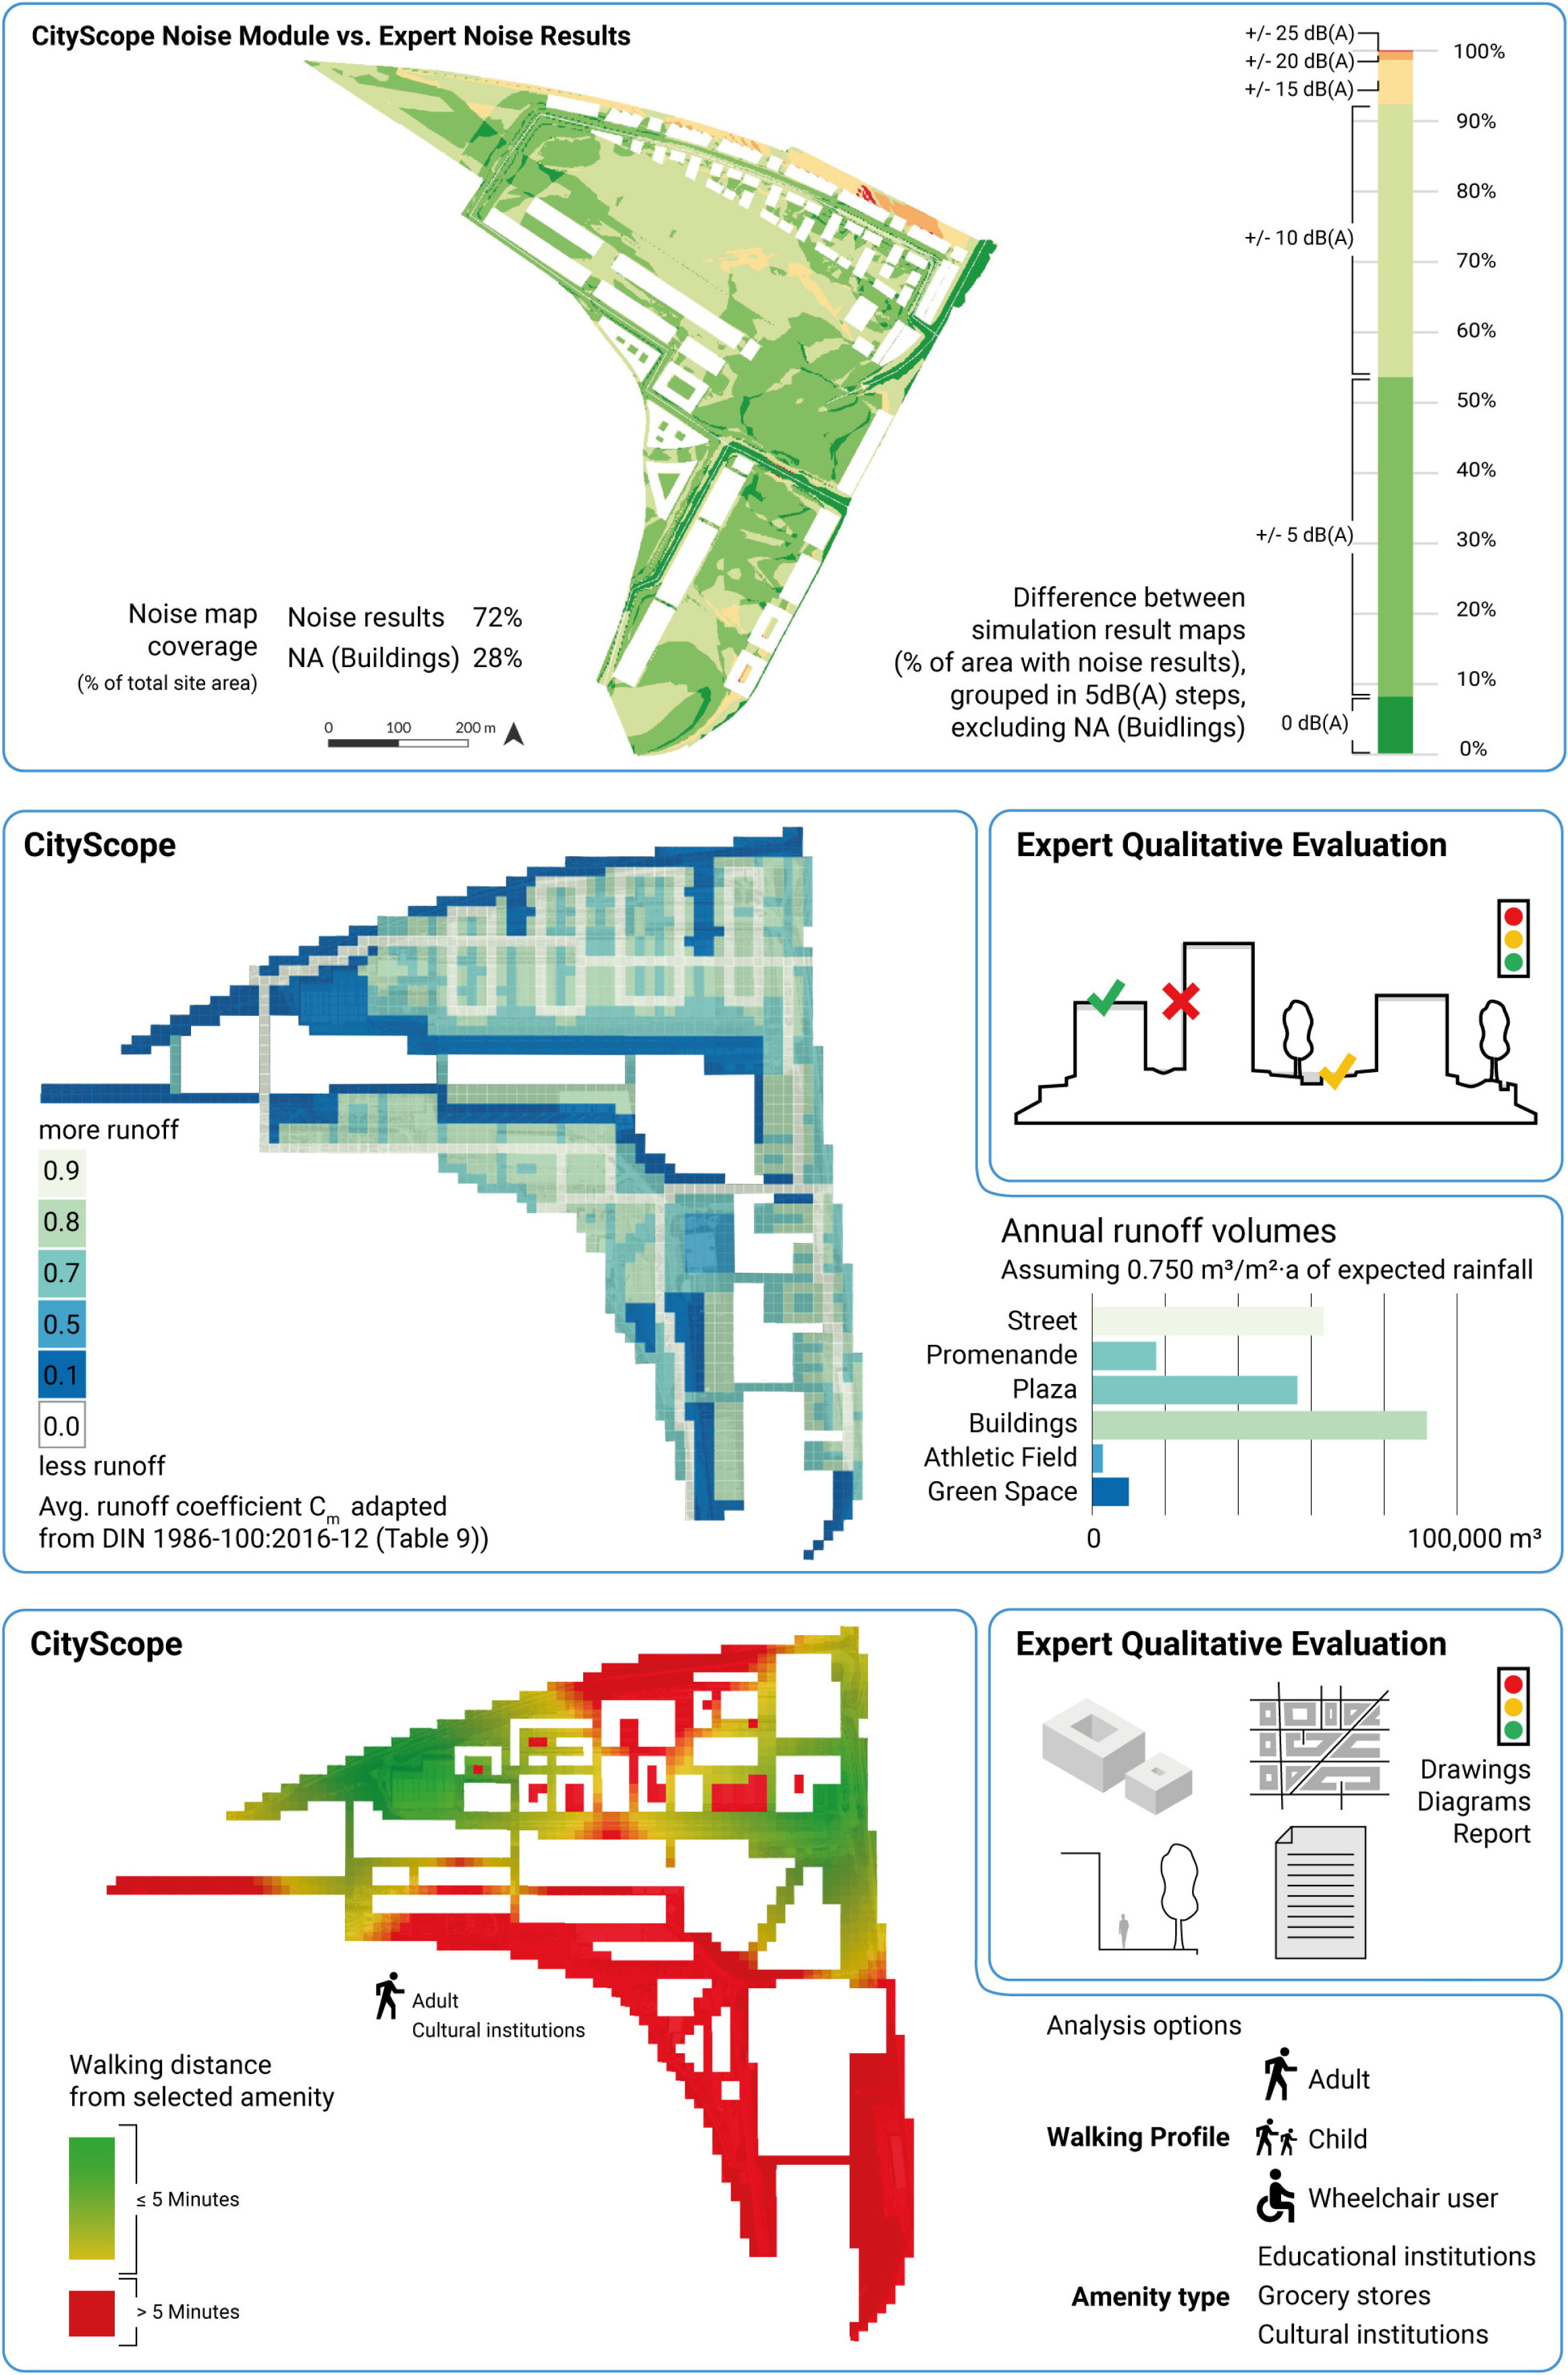
\includegraphics[width=.7\textwidth]{chapters/transformation/grasbrook/figures/grsbrk0.png}

            \end{center}
            \caption{
                Analytic modules developed for the Grasbrook competition (From the top):
                (i) CityScope noise analysis result compared to experts' analysis for the winning competition entry; (ii) CityScope results of runoff coefficients. Estimated annual runoff volumes m\textsuperscript{3} by surface type. Upper Right: Qualitative evaluation used to assess schematic map submissions; (iii) Walkability calculations results for user type `adult' and `cultural institutions'. Areas in green show the travel distance below the threshold of a five-minute walk. Upper Right: Qualitative evaluation method used to assess submission materials, including schematic maps, explanatory sketches, and pictograms.
            }
            \label{fig:grasbrook_results}
        \end{figure}

        \subsubsection{Noise Module}
        {
            Noise emission is a key concern in urban-design and city-planning. Grasbrook site is situated near major transit arteries, highways, railways, as well as an industrial port area, making the appropriate estimation of acoustic impact, a crucial item in the evaluation of design proposals \cite{e19}. In conventional planning procedures, noise performance of design proposals is usually possible only through expert evaluation in advanced stages, sometimes years after the initial competition phase has been concluded. In contrast, the noise module developed for the Grasbrook CityScope was able to model noise propagation throughout the design area in near real-time.
            \newline
            This module considers noise emitters, such as large streets and adjacent railway lines, on the basis of predicated traffic loads. It uses software developed by the French Institute of Science and Technology for Transport, Development and Networks \cite{bgppf19}, which is based on a simplified implementation of the French standard for urban noise propagation, NMPB-08 \cite{n11}. When designers interact with the CityScope grid, the noise simulation tool extracts building footprints and calculates a 2D noise distribution map. The noise emitted by simulated traffic on streets and railways is propagated through the design area, taking into account the diffractions and reflections caused by the buildings.
            \newline
            \textbf{Evaluation and Validation:} In order to evaluate the noise module accuracy, the CityScope noise module were compared to results retrieved from an established noise modeling consultancy. Figure \eqref{fig:grasbrook_results} presents the results of the analysis of the winning competition entry performed with the CityScope tool compared to the results delivered by the external consultancy. Visually, both noise maps shows similar dispersal patterns. When rasterizing both result sets, a differential map is computed to locate and visualize the differences in estimated noise levels. This differential map indicates that the total area of noise level differences greater than 10dB are below 7.5\% of the design area, whereas 53\% of the design area show deviations of max 5db. The remaining 39.5\% of the design area shows deviations between 5 and 10 dB.
            \newline
            Studies have shown that different experts evaluating noise using different national methods create results which deviate by 10 to 15dB \cite{nw05}. In this case, a main cause for the deviation results is the different calculation methods used by the CityScope and the external consultancy, which differ in the standard metrics utilized\footnote{Simplified implementation of the French NMPB-08 standard for CityScope vs. German RLS 90 standard for road noise sources and unspecified methods for propagation calculation Consultancy}. Moreover, technical differences and input assumptions influence the definition of noise modeling accuracy, such as:
            (i) Rasterized CityScope input format leads to simplifications of the design proposal, from building footprints to a grid-based input;
            (ii) Experts added higher noise levels to context-specific locations (e.g., bridges over the Elbe River);
            (iii) French and German standards use different annotation scales for noise levels;
            (iv) CityScope delivers a composite day, evening and night index (LDEN) while the method deployed by the external consultancy indexes for daytime only.
            \newline
            As a general trend, the results delivered by the CityScope generally show lower noise levels than the ones delivered by the external consultancy. Still, a proportional behavior and distribution of the noise levels underline the applicability of the tool for real-time noise modeling.
        }


        \subsubsection{Storm-water Module}
        {
            As in many other parts of the city of Hamburg, the Grasbrook district is vulnerable to flooding caused by heavy rainfall events and sea-level rise. The HafenCity Hamburg GmbH requested a storm-water module in order to evaluate the synergies between green storm-water infrastructure, comfortable microclimatic conditions, and the functional requirements for landscape design. This module calculates the surface runoff from each cell in the CityScope grid, and combines it to an annual storm-water runoff analysis. Each cell of the grid contains data about the surface type (e.g., building, street, open-space) and each type is assigned a runoff coefficient\footnote{The runoff coefficients were adapted from Table 9 of DIN 1986-100:2016-12 \cite{e16}.}. The $m^2$ area of each cell is multiplied by the runoff coefficient and by the annual rainfall $m^3/m^2*a$.
            \newline
            \textbf{Evaluation and Validation:} Today, most experts rely on schematic blueprints or renderings to evaluate storm-water potential. These schematics often lack the information necessary to evaluate the submissions beyond a baseline qualitative assessment. CityScope storm-water module uses standardized measures of surface permeability and infiltration potential, in order to estimate cumulative annual runoff volumes. While expert analysis for water-cycles usually involves a tricolor rating system, CityScope enables a quantitative comparison of the design submissions in their entirety, while still supporting qualitative assessments.
            \newline
            Nevertheless, some spatial aspects were not consistently present in all design submissions, for example: (i) Topography within the area; (ii) Directional flows within the storm-water network, and (iii) Location and size of infrastructure, such as infiltration, retention, water treatment facilities, or neighborhood cistern. Consequently, the Grasbrook version of the storm-water module did not include these aspects, either. Already in its current form, the storm-water module can deliver a valuable quantitative comparison of the designs in regards to the ratio of green and open-space, as well as annual runoff projections from differentiated surface types.
        }

        \subsubsection{Walkability Module}
        {
            Walkability is a key parameter in the evaluation of urban districts and neighborhoods design \cite{carr1969city, krier1979urban}. Human-centred urban-design promotes the development of neighborhoods that well-function without broad usage of motorized vehicles; In order to prevent unnecessary traffic and subsequent negative environmental impacts, basic amenities and socio-spatial infrastructure need to be accessible to all local residents within a minimal walking distance \cite{banerjee2011companion}. In order to identify the distribution of services and amenities during early urban-design processes, an analytic module was devised to calculate the 5-minute walkshed of a subset of amenities, such as educational, cultural or retail. The tool implements a standardized isochrone calculation using the walkable street network, a common method utilized in walkability and accessibility research \cite{dp20, dwp17}.
            \newline
            \textbf{Evaluation and Validation:} While the expert analysis was based on a qualitative evaluation of the pedestrian network, CityScope numerically calculated the accessibility based on the street network morphology in the proposal. Specifically, the module calculated accessibility to-and-from different amenity types, using three main trip profiles: adult, child, and wheelchair user. Each of the walking profiles includes an average speed and a list of surfaces through which they can traverse comfortably; For example, wheelchair users might not be able to pass through streetscape involving stairs or steep slopes. The walkability calculation for each amenity type, and each walking profile, is performed using a flood-fill calculation performed by Dijkstra's shortest path algorithm on the CityScope grids \cite{eldg14}. The CityScope walkability module enables quantitative analysis of accessibility, complementing the mostly qualitative interpretation provided by the mobility and transportation experts.
        }

        \subsubsection{GFA Module}
        {
            A common indicator for the economic and spatial feasibility of urban-design is the Gross Floor Area (GFA) \cite{fcc18}. Balancing between economic profitability (production of marketable real-estate) and spatial quality (openness, view, visibility), is a key in urban-design processes. The definition of GFA do not only affect physical parameters (e.g., distribution of light and shadow) but also local logistics and supplies, as well as the provisioning of social infrastructure (e.g., day-care or medical facilities). The CityScope GFA module calculates the aggregated GFA in square meters in respect to the classification of building-use defined in the competition brief.
            \newline
            \textbf{Evaluation and Validation:} Given the simplification imposed by CityScope grid rasterization (see Section \eqref{subsec:types_system}), the accuracy of this module depends on the granularity of the design submission, and their adherence to parallel lines, or right angles. Naturally, freeform-designs achieve lower accuracy in GFA analysis than designs based on rectangular blocks, due to deviations in the calculated floor area. In order to determine the accuracy of the module, calculations were compared with expert evaluation reports which include a cross-check of designed volumes against the definitions made by the competition brief \cite{e19}. The main land-use categories, `Commercial' and `Residential,' correspond closely with the same use types in the competition brief, whereas the CityScope category `Other' roughly translates to `Special use,' which includes cultural, educational, and sports usages.
            \newline
            Differences in type classification between CityScope and the competition brief, the transformation of the designs to the CityScope grid, and subjective data entry, contributed to misalignment in GFA module results, compared to experts evaluation. In 7 of 8 cases, the absolute difference ranged from 1\% to 27\%, with an average of absolute difference of 14\%. For one competition entry, the absolute difference was 170\% for `Other' due to the user's interpretation of non-standard mixed use types as `Other' rather than primarily `Residential' or `Commercial'. In future use-cases, a GFA module should be designed in a more flexible way, so that it could match GFA requirements of a competition brief.
        }
    }

    \subsection{Discussion}
    {
        The Grasbrook project was the first opportunity to involve CityScope system, including frontend, modules, cityIO, and other components, in a real-world design competition process.
        CityScope Grasbrook was implemented for two different use-cases: (i) Designers and planners developing design proposals during the competition, and (ii) Competition juries evaluation of these design proposals. This section evaluates the usage of CityScope for each of the two use-cases.

        \subsubsection{Strengths}
        {
            The time and cost of obtaining expert analysis is a major obstacle in the creation of feasible, sustainable and well-balanced urban-design proposals. CityScope compensates this deficit by delivering data-driven and real-time results during the design process. Moreover, CityScope architecture promotes a single data input (CityScope Grid, see Section \eqref{sec:cityscope_architecture}) which is shared across the different analytic modules. This structure avoids inputting design schemes into separated software applications, or carry out time-consuming data transfer and reformatting.
            \newline
            Additionally, CityScope provides a standardized assessment of both spatial, environmental, and social qualities of urban-design proposals. It enables an objective assessment of completely different designs, which is particularly useful when evaluating several proposals under the same set of criteria. Simplified interaction and standard visualization make the comparison of proposals substantially easier, for both the design juries and designers themselves. CityScope's standardized data format, and open-source modules provide transparency in the process of analysis and assessment, and allow technical consensus amongst domain-experts.
        }

        \subsubsection{Weaknesses}

        {
            The accuracy of the analytic modules remains a scientific and methodological challenge. Designers, juries, developers, or investors depend on clear indications and relative reliability compared to well-established methods of evaluation. While validation was preformed for the noise and rainwater modules, the discrepancy of scientific models, methodology, and data schemes, challenges an in-depth validation and refinement of other modules.
            \newline
            Even though one single data structure (CityScope Grid) can be more time efficient compared to several data inputs and separated applications, the current tool required that the designs would be manually uploaded. This was accomplished by importing multiple layers of geospatial information (e.g., existing buildings, site restrictions), as well as rasters of the first round designs, to allow users to translate them into CityScope grids. To make the input and translation process easier, users expressed interest to import data formats common for their preferred design software or competition submission files (e.g., DWG, RVT, IFC). In the future, such data conversion pipeline could be added to CityScope for automatic CAD and BIM data conversion.
        }

        \subsubsection{Opportunities}
        {
            A key benefit of CityScope is its capacity to run different types of analysis at the same time. In this respect, it has greater analytic power than evaluations which only consider one dimension at a time. By changing the layout of a plot or a building in one specific setting, impacts on many different other KPIs and metrics can be observed. By cross-connecting the various analytic modules, new inputs will simultaneously change and update other performance layers.
            \newline
            Validated CityScope modules and open-source development, can ensure that the evaluation of design proposals will not be delivered as rigid `black-box' solutions. Open-source development makes non-generic modules (such as site-specific analysis) easily adaptable to other future scenarios, and allows for better validation by the scientific community. As a digital online tool, CityScope has the potential to facilitate communication and dialogue with larger stakeholders groups, neighborhood communities, local initiatives, or academia.
        }

        \subsubsection{Threats}
        {
            The introduction of new processes and technologies can be accompanied by scepticism and rejection from its target audience. Designers tend to have well-established workflows, especially in the stressful context of design competition projects, where they rely on conceptual and technical traditions adopted over years. Similarly, jurors might not welcome the appearance of new decision-support systems: discrepancies and conflicts between expert judgement and algorithmic analysis may occur, and might be considered a disruption of established power-structures and political dominance. It is therefore critical to properly position CityScope-like tools as decision-support systems, not a replacement for experts and community discussion.
        }

    }

    \subsection{Conclusion}
    {
        CityScope Grasbrook was an initial attempt to \textit{`reinvent the competition'}, by offering an open-ended digital platform for design analysis and evaluation. This project has demonstrated its applicability for high-stake international urban-design competition, by effectively supporting the decision making of (i) Designers and planners in the process of developing sustainable urban-designs proposals, and (ii) Competition juries mandated for the evaluation of the final proposals. To both, CityScope provided instant assessment and analytic evidence via multiple key metrics.
    }
}























    %%%%%%%%%%%%%%%%%%%%%%%%%%%%%%%%%%%%%%%%%%%%%%%%%%

    \section{Discussion: UHCI for Urban Transformation}
     {
      This chapter explored the core design principles of the CityScope platform, and the ways it supports several urban transformation processes in real-world planning context. It reviewed the CityScope ecosystem, with an emphasis on the interoperability of data and analysis using the CityScope Schema, cityIO, backend modules, and frontend interfaces.
      Most use-cases in this chapter demonstrated the way CityScope supports the analysis of rather traditional urban indicators, such as accessibility, energy, urban-from, or vehicular mobility. Yet beyond these metrics, CityScope aims to asses and predict more subtle urban indicators, such as human interaction and social dynamics. The next chapter, \textit{Prediction} \eqref{ch:prediction}, looks into CityScope models and modules used to provide predictive analysis on more implicit matrices. It focuses on questions of movement, social dynamics, as well as the appearance of the city, as proxies to the evaluation of changes in the built environment.
     }

}